% ----------------------------------------------------------------
% AMS-LaTeX Paper ************************************************
% **** -----------------------------------------------------------
\documentclass[12pt]{amsart}
\usepackage{graphicx}
\usepackage{amsmath,bm,amssymb}
\usepackage{color}

\hoffset=-0.5in
\textwidth=6in
%\swapnumbers
\newtheorem{theorem}{Theorem}[section]
\newtheorem{lemma}[theorem]{Lemma}
\newtheorem{prop}[theorem]{Proposition}
\newtheorem{cor}[theorem]{Corollary}

\theoremstyle{definition}
\newtheorem{defn}[theorem]{Definition}
\newtheorem{example}[theorem]{Example}

\theoremstyle{remark}
\newtheorem{rem}[theorem]{Remark}

\numberwithin{equation}{section}
% MATH -----------------------------------------------------------
\newcommand{\norm}[1]{\left\Vert#1\right\Vert}
\newcommand{\abs}[1]{\left\vert#1\right\vert}
\newcommand{\set}[1]{\left\{#1\right\}}
\newcommand{\Real}{\mathbb R}
\newcommand{\eps}{\varepsilon}
\newcommand{\To}{\longrightarrow}
\newcommand{\BX}{\mathbf{B}(X)}
\newcommand{\F}{\mathcal{F}}
\newcommand{\mean}[1]{{\langle #1\rangle}}
\newcommand{\alert}[1]{\fbox{#1}}
\newcommand{\ip}[2]{{\langle #1,#2\rangle}}
\newcommand{\1}{\mathbf 1}
\newcommand{\Var}{{\operatorname{Var}}}
\renewcommand{\Im}{{\mathcal I}}
\newcommand{\eqfd}{\stackrel{f.d.}{=}}
\newcommand{\rr}{\mathbb R}
\newcommand{\E}{\mathbb E}
\newcommand{\R}{\mathbb R}
\newcommand{\ttheta}{\mbox{\boldmath$\theta$}}
\newcommand{\X}{{\mathbf X}}
\newcommand{\noi}{\noindent}

% ----------------------------------------------------------------
\begin{document}
\sloppy
\title[Fitting ARTFIMA time series]{Parameter estimation for ARTFIMA time series}

\author{Farzad Sabzikar}
\address{Farzad Sabzikar, Department of Statistics,
Iowa State University, Ames, IA 50011}
\email{sabzikar@iastate.edu}
\urladdr{http://sabzikar.public.iastate.edu/}



\author{Ian McLeod}
\address{Ian McLeod, Department of Statistics,
Western University, Canada}
\email{aim@stats.uwo.ca}

\author{Mark M. Meerschaert}
\address{Mark M. Meerschaert, Department of Statistics and Probability,
Michigan State University, East Lansing MI 48823}
\email{mcubed@stt.msu.edu}
\urladdr{http://www.stt.msu.edu/users/mcubed/}

\thanks{MMM was partially supported by ARO MURI grant W911NF-15-1-0562 and NSF grants DMS-1462156 and EAR-1344280.}



% ----------------------------------------------------------------
\begin{abstract}
The ARTFIMA model applies a tempered fractional difference to the standard ARMA time series.  This paper develops parameter estimation methods for the ARTFIMA model, and demonstrates a new R package.  Several examples illustrate the utility of the method.
\end{abstract}

\maketitle

\section{Introduction}\label{sec1}
The autoregressive tempered fractionally integrated moving average (ARTFIMA) time series model was introduced in Meerschaert et al.\ \cite{Meerschaertsabzikarkumarzeleki}, see also Sabzikar et al.\ \cite{TFC}.  The ARTFIMA model extends the TFI model from Giraitis et al.~\cite{giraitis}, who note that tempered fractionally integrated times series exhibit {\it semi-long range dependence}:  Their covariance function resembles long range dependence for a number of lags, depending on the tempering parameter, but eventually decays exponentially fast.  
%The TFI model is mathematically equivalent to the first order generalized autoregressive (GAR) model of Peiris \cite{Peiris}.
In this paper, we develop the mathematical foundation for ARTFIMA parameter estimation, and present a new R package {\tt artfima} to fit data.  Several examples from finance, geophysics, turbulence, and climate illustrate the fitting procedure, and the utility of the ARTFIMA model.

There are three reasons to consider the ARTFIMA model.  The first is mathematical.  The ARFIMA model without tempering is challenging to analyze, since the covariance function is not summable.  The ARTFIMA model, however, has a summable covariance function, and hence its properties can be derived using standard methods.  Since the tempering parameter can be made as small as we like, the {\it mathematically more tractable} ARTFIMA model can fit data that is usually modeled using the ARFIMA model.

The second reason is statistical.  The power spectral density function of the ARFIMA model is asymptotically a power law that diverges as the frequency approaches zero.  However, in many applications, data fit this power law model only up to a low frequency cutoff, after which the observed spectral density remains bounded.  A classical example is turbulence: According to the Kolmogorov model, the spectral density is proportional to $k^{-5/3}$ in the inertial range, where $k$ is the frequency.  Since the observed power spectrum in actual turbulence data typically remains bounded as $k\to 0$, the ARTFIMA model provides a {\it better fit}.  See \cite{Meerschaertsabzikarkumarzeleki} for additional discussion.

The third reason is conceptual.  The ARTFIMA model with any order of tempered fractional differencing is a {stationary} time series.  It has now become common in many applications to model long range dependence using either an ARFIMA model or a fractional Brownian motion. A fractional Brownian motion with Hurst index $H=1/3$ satisfies the Kolmogorov model, as does an ARFIMA with $d=5/6$.  Both of these models have stationary increments.  However, typical applications involve data that most scientists believe form a stationary sequence.  The ARTFIMA model provides a more suitable {\it stationary} time series model for such data.

%Fractionally integrated time series have proven useful for modeling long range dependence \cite{BrockwellDavisTSTM,koul}.  Recently, a model extension has been proposed based on tempered fractional calculus \cite{TFC}.  The autoregressive fractionally integrated moving average (ARFIMA) time series $X_t=\Delta^d Y_t$ where $\Delta^d=(I-B)^d$ using the backward shift operator $BY_t=Y_{t-1}$, and $Y_t$ is a classical autoregressive moving average (ARMA) time series.  Similarly, the autoregressive tempered fractionally integrated moving average (ARTFIMA) time series is defined by $X_t=\Delta^{d,\lambda} Y_t$ where $Y_t$ is an ARMA time series, and the tempered fractional difference operator $\Delta^{d,\lambda} =(I-e^{-\lambda}B)^d$.  The ARTFIMA model is a short range dependent time series that nonetheless exhibits {\it semi-long range dependence} \cite[Eq.\ (30)]{TFC}: For small values of the tempering parameter $\lambda>0$, the spectral density grows like a power law at low frequencies, but remains bounded as the frequency tends to zero.  The same behavior is commonly observed in geophysical turbulence, and it was demonstrated in \cite{Meerschaertsabzikarkumarzeleki} that the ARTFIMA model provides a good fit to such data.  In particular, the ARTFIMA model reproduces Kolmogorov scaling in the inertial range, but also fits the low frequency periodogram.
%
%Fractional calculus was invented by Leibnitz, and recently has found numerous applications in science and engineering \cite{FCbook,MetzlerK,MetzlerKlafter,MillerRoss,oldham,Samko}.  Fractional derivatives are the limits of fractional difference quotients \cite[Proposition 2.1]{FCbook}, and similarly, tempered fractional derivatives are the limits of tempered fractional difference quotients \cite[Proposition 7.8]{FCbook}.   Fractional Brownian motion was invented by Kolmogorov \cite{KolmogorovFBM} as a model for turbulence, using a spectral representation. Mandelbrot and Van Ness \cite{MV68} gave the process its name, and wrote its moving average representation, a fractional integral in time of a continuous parameter Gaussian white noise.  The simplest ARFIMA time series, a fractionally integrated Gaussian white noise, can be viewed as a fractional Brownian motion sampled at integer time points.  Recently, a tempered fractional Brownian motion has been developed, as the tempered fractional integral of a Gaussian white noise \cite{TFBM,TFI}.   A tempered fractionally integrated Gaussian white noise can be obtained by sampling tempered fractional Brownian motion at integer time points.

%This paper develops the basic theory and parameter estimation methods for ARTFIMA time series.  Since these time series are mathematically short range dependent, the methods are classical.  However, we develop explicit formulae needed for practical applications, including geophysical turbulence.  This paper also documents an R package called {\tt artfima} that is freely available on CRAN.  An example application is included here to demonstrate the software, and to rigorously verify the results in \cite{Meerschaertsabzikarkumarzeleki}.


\section{The ARTFIMA model}\label{sec4}
In this section, we define the ARTFIMA model, and develop some basic results including causality, invertibility, the covariance function and spectral density.

The tempered fractional difference operator is defined by:
\begin{equation}\label{eq:TFdiffDef}
\Delta^{d,\lambda} f(x)=(I-e^{-\lambda }B)^d f(x)=\sum_{j=0}^\infty \omega^{d,\lambda}_{j}f(x-j)
\end{equation}
where $d>0$, $\lambda>0$, $BX_t = X_{t-1}$ is the shift operator, and
\begin{equation}\label{omegadef}
\omega^{d,\lambda}_{j}:=(-1)^j\binom d  je^{-\lambda j}\quad\text{where}\quad \binom d  j=\frac{\Gamma(1+d)}{j!\Gamma(1+d-j)}
\end{equation}
using the gamma function $\Gamma(d)=\int_{0}^{\infty}e^{-x}x^{d-1}\ dx$. Using the well-known property $\Gamma(d+1)=d\Gamma(d)$, we can extend \eqref{eq:TFdiffDef} to non-integer values of $d<0$.  By a common abuse of notation, we call this a tempered fractional integral.
%Then we have
%\[D^{d,\lambda} f(x)=\lim_{h\to 0} h^{-d} \Delta^{d,\lambda}_{1}_h f(x)\]
%whenever $f$ and its derivatives up to order $n>1+d$ exist and are absolutely integrable \cite[Theorem 5.1]{TFC}.
If $\lambda=0$, then equation \eqref{eq:TFdiffDef} reduces to the usual fractional difference operator. See \cite{TFI,TFC} for more details.

\begin{defn}\label{defn:artfima general definition}
The discrete time stochastic process $\{X_t\}_{t\in{\mathbb Z}}$ is called an {\it autoregressive tempered fractional integrated moving average} time series, denoted by ARTFIMA$(p,d,\lambda,q)$, if $\{X_t\}_{t\in\mathbb{Z} }$ is a stationary solution with zero mean of the tempered fractional  difference equations
\begin{equation}\label{eq:artfima general definition}
\Phi(B)\Delta^{d,\lambda} X_{t}=\Theta(B)Z_{t},
\end{equation}
where $\{Z_t\}_{t\in\mathbb{Z} }$ is a white noise sequence (i.i.d.\ with ${\mathbb E}[Z_t]=0$ and ${\mathbb E}[Z_t^2]=\sigma^2$), $d\notin{\mathbb Z}$, $\lambda>0$, and $\Phi(z)=1-\phi_1 z-\phi_2 z^2-\ldots -\phi_{p}z^{p}$, and $\Theta(z)=1+\theta_1 z+\theta_2 z^2+\ldots +\theta_{q}z^{q}$ are polynomials of degrees $p,q\geq 0$ with no common zeros.
\end{defn}

\begin{rem}
It follows from Definition \ref{defn:artfima general definition} that $X_{t}$ is ARTFIMA$(p,d,\lambda,q)$ if and only if $Y_t=\Delta^{d,\lambda} X_t$ is   an ARMA$(p,q)$ time series
\begin{equation*}\label{eq:ARMA}
Y_t - \sum_{j=1}^p \phi_j Y_{t-j}=Z_t+\sum_{i=1}^q \theta_i Z_{t-i}
\end{equation*}
where $\{Z_t\}_{t\in\mathbb{Z} }$ is a white noise sequence.


\end{rem}

{\bf Assumption A:}
In this paper, we always assume the polynomials $  \Phi(\cdot) $ and $ \Theta(\cdot) $ have no common zeros and
\begin{equation}\label{eq:assumption a}
\big|\Phi(z)\big|>0\quad\text{and}\quad \big|\Theta(z)\big|>0
\end{equation}
for $|z|\leq 1$.


\begin{theorem}\label{th2.3}
Suppose that $\{X_t\}_{t\in\mathbb{Z}}$ is an ARTFIMA$(p,d,\lambda,q)$ time series that satisfies Definition \ref{defn:artfima general definition}
with polynomials $  \Phi(\cdot) $ and $ \Theta(\cdot) $ satisfy under assumption A. Then:


\noi(a) $X_{t}$ is causal, i.e.,
$
X_{t}=\sum_{j=0}^{\infty}a^{-d,\lambda}_{j}Z_{t-j},
$
where $\sum_{j=0}^{\infty}\big|a^{-d,\lambda}_{j}\big|<\infty$; and
\noi(b) $X_{t}$ is invertible, i.e.,
$
Z_{t}=\sum_{j=0}^{\infty}c^{d,\lambda}_{j}X_{t-j},
$
where $\sum_{j=0}^{\infty}\big|c^{d,\lambda}_{j}\big|<\infty$.

\end{theorem}

The proofs of all the results in this paper can be found in the Appendix.


In order to compute the covariance function of the ARTFIMA$(p,d,\lambda,q)$ process $X_t$, we first recall a useful computational form of the spectral density for the ARMA$(p,q)$ process $\Phi(B)U_{t}=\Theta(B)Z_{t}$, where $Z_t$ is a white noise with ${\mathbb E}[Z_t^2]=\sigma^2$.   Under \eqref{eq:assumption a}, $\Phi(x)$ can be written
\begin{equation*}
\Phi(x)=\prod_{j=1}^{p}(1-\rho_j x),
\end{equation*}
where $\rho_1,\ldots,\rho_p$ are the complex numbers such that $|\rho_n|<1$ for $n=1,2,\ldots,p$ (see Sowell \cite[Section 4]{sowell1}). Then the spectral density of $U_t$ is
\begin{equation*}
\begin{split}
f_{U}(\nu)&=\frac{\sigma^2}{2\pi}\frac{\Big|\Theta(\omega)\Big|^2}{\Big|\Phi(\omega)\Big|^2}\\
&=\frac{\sigma^2}{2\pi}\Big|\Theta(\omega)\Big|^2\prod_{j=1}^{p}(1-\rho_j \omega)^{-1}(1-\rho_j \omega^{-1})^{-1},
\end{split}
\end{equation*}
where $\omega=e^{-i\nu}$. According to Sowell \cite[Section 4]{sowell1}, the spectral density of $U_t$ can also be written as
\begin{equation}\label{eq:hUk}
f_{U}(\nu)=\frac{\sigma^2}{2\pi}\sum_{l=-q}^{q}\psi(l)\omega^l \sum_{j=1}^{p}\omega^p
\zeta_{j}\Big[\frac{{\rho_j}^{2p}}{(1-\rho_j\omega)}-\frac{1}{(1-\rho_j^{-1}\omega)}\Big],
\end{equation}
where
\begin{equation*}
\psi(l)=\sum_{s=\min[0,l]}^{\max[q,q+l]}\theta_{s}\theta_{s-l},
\end{equation*}
and
\begin{equation*}
\zeta_{j}=\frac{\sigma^2}{2\pi}\Big[\rho_j\prod_{i=1}^{p}(1-\rho_i\rho_j)\prod_{m\neq j, 1\leq m \leq p}(\rho_j-\rho_m)\Big]^{-1}.
\end{equation*}


The next theorem gives the spectral density and explicit form of the covariance function of ARTFIMA$(p,d,\lambda,q)$.

\begin{theorem}\label{thm:Proprties}
Suppose that $\{X_t\}_{t\in\mathbb{Z}}$ is an ARTFIMA$(p,d,\lambda,q)$ time series that satisfies Definition \ref{defn:artfima general definition}, and that \eqref{eq:assumption a} holds.  Then:
\begin{itemize}
\item  [(a)] $\{X_t\}$ has the spectral density
  \begin{equation}\label{eq:spectraldensity}
   f_X(\nu)=\frac{\sigma^2}{2\pi}\frac{\left|\Theta(e^{-i\nu})\right|^2}{\left|\Phi(e^{-i\nu})\right|^2}\ \left|1-e^{-(\lambda+i\nu)}\right|^{-2d}
  \end{equation}
  for $-\pi\leq \nu\leq \pi$.
  \item [(b)] The covariance function of $\{X_t\}$ is
  \begin{equation*}
\begin{split}
\gamma_X(k)
%&=\int_{-\pi}^{\pi}h_{X}(\nu)e^{i\nu k}\ d\nu\\
%&=\frac{\sigma^2}{2\pi}\int_{-\pi}^{\pi}\Bigg[\sum_{l=-q}^{q}\sum_{j=1}^{p}\psi(l)\zeta_{j}\Big[\frac{{\rho_j}^{2p}}{(1-\rho_j\omega)}-\frac{1}{(1-\rho_j^{-1}\omega)}\Big]\\
%&\quad\quad\quad\Big(1-e^{-(\lambda+i\nu)}\Big)^{-d}\Big(1-e^{-(\lambda-i\nu)}\Big)^{-d}\omega^{p+l}\Bigg]e^{i\nu k}\ d\nu\\
&=\frac{\sigma^2}{2\pi}\sum_{l=-q}^{q}\sum_{j=1}^{p}\psi(l)\zeta_{j}C(d,\lambda,k-l-p,\rho_j),
\end{split}
\end{equation*}
using the notation in \eqref{eq:hUk}, where
\begin{equation}\label{eq: C lambda computation definition}
\begin{split}
&C(d,\lambda,h,\rho)\\
&=\rho^{2p}\sum_{m=0}^{\infty}
\frac{\rho^{m}e^{-\lambda(h-m)}\Gamma(h-m+d)\ {_2F_1(d;h-m+d;h-m+1;e^{-2\lambda})}}{\Gamma(d)\Gamma(h-m+1)}\\
&\quad +\sum_{n=1}^{\infty}\frac{\rho^{n}e^{-\lambda(h+n)}\Gamma(h+n+d)\ {_2F_1(d;h+n+d;h+n+1;e^{-2\lambda})}}{\Gamma(d)\Gamma(h+n+1)},
\end{split}
\end{equation}
\end{itemize}
where the Gaussian hypergeometric function
\begin{equation*}
\begin{split}
_2F_1(a;b;c;z)&=\sum_{j=0}^{\infty}\frac{\Gamma(a+j)\Gamma(b+j)\Gamma(c)}{\Gamma(a)\Gamma(b)\Gamma(c+j)\Gamma(j+1)}z^j\\
&=1+\frac{a\cdot b}{c\cdot 1}z+\frac{a(a+1)b(b+1)}{c(c+1)\cdot 1\cdot 2}z^{2}+\cdots
\end{split}
\end{equation*}
is defined for all complex numbers $a$ and $b$, all complex $|z|<1$ and real $c$ not a negative integer.
%As $c\to -n$, a negative integer, we have
%\begin{equation*}
%\begin{split}
%\lim_{c\to -n}\frac{_2F_1(a;b;c;z)}{\Gamma(c)}&=a(a+1)\ldots(a+n)b(b+1)\ldots(b+n)\\
%&\quad\cdot z^{n+1}\ _2F_1(a+n+1;b+n+1;n+2;z).
%\end{split}
%\end{equation*}
%Hence when $c=-n$ we define $_2F_1(a;b;c;z)$ using this limit.   We refer the reader to \cite[Chapter 9]{Gradshteyn} for more details about the Gaussian hypergeometric function.



\end{theorem}


%\subsection{Tempered fractional noise}
An important special case of the ARTFIMA$(p,d,\lambda,q)$ process is when $p=q=0$. In this case, we have
\begin{equation}\label{ART}
X_t = (1- \ e^{-\lambda} B)^{-d} Z_{t}  =
\sum_{k=0}^{\infty} \omega^{-d,\lambda}_k Z_{t-k}, \qquad t \in \mathbb{Z}
\end{equation}
where $\omega^{-d,\lambda}_k$ is given by \eqref{omegadef}.
The TFI$(d,\lambda)$ model in \eqref{ART}  appeared in  Giraitis et al.~\cite{giraitis}, who noted
that for small $\lambda >0$, $X_t$ has a covariance function
that resembles the covariance function of a long memory model for an arbitrarily large number of lags, but
eventually decays exponentially fast. Following \cite{giraitis}, we say that $X_t$ exhibit {\it semi-long range dependence}.
Meerschaert et al.~\cite{Meerschaertsabzikarkumarzeleki} apply the TFI$(d,\lambda)$ model
\eqref{ART} to turbulent water velocity data from the Great Lakes. 
%Peiris \cite{Peiris} has proposed a generalized autoregressive GAR$(1)$ time series model $(1-\beta B)^d V_t=Z_t$ for applications in finance, where $|\beta|<1$ and $BZ_{t}=Z_{t-1}$ is the backward shift operator. Taking $\beta=e^{-\lambda}$ we obtain the model \eqref{ART}. Shitan and Peiris \cite{Peiris2} considered the maximum likelihood estimator (MLE)
%and Whittle's estimator for parameters in GAR(1) model.
%In the next section, we consider the parameter estimation of ARTFIMA$(p,d,\lambda,q)$.




%
%\begin{theorem}\label{thm:interesting property of covariance}
%Let $W_t$ be a tempered fractional noise, i.e., an ARTFIMA$(p,d,\lambda,q)$ time series as in Definition \ref{defn:artfima general definition} with $p=q=0$, $d\notin{\mathbb Z}$, and $\lambda>0$. Then
%\begin{equation}\label{eq:interesting property of covariance}
%\sum_{k=0}^{+\infty}\big|\gamma_W(k)\big|<\infty\quad\quad \text{and}\quad\ \sum_{k=-\infty}^{+\infty}\gamma_W(k)=\sigma^2(1-e^{-\lambda})^{-2d}.
%\end{equation}
%\end{theorem}
%
%
%%\begin{rem}
%%If $W_t$ is a fractional noise, ARTFIMA$(0,d,0,0)$, we have:
%%\begin{equation*}\begin{split}
%%\sum_{k=0}^{+\infty}\big|\gamma(k)\big|<\infty\quad\quad \text{and}\quad\ \sum_{k=-\infty}^{+\infty}\gamma(k)=0&\quad\quad \text{for $-\frac{1}{2}<d<0$;}
%%\end{split}\end{equation*}
%%and
%%\begin{equation*}\begin{split}
%%\sum_{k=0}^{+\infty}\big|\gamma(k)\big|=\infty&\quad\quad \text{for $0<d<\frac{1}{2}$,}
%%\end{split}\end{equation*}
%%see Proposition 3.2.1 in \cite{koul}.  This is consistent with Theorem \ref{thm:interesting property of covariance}, as the last term in \eqref{eq:interesting property of covariance} tends to zero or infinity, depending on the sign of $d$, as $\lambda\to 0$.
%%\end{rem}
%
%
%%The next lemma gives the spectral representation of the ARTFIMA $(0,d,\lambda,0)$. We will use this lemma in the next section.
%%\begin{lemma}\label{lem:spectralrepresntation ARTFIMA}
%%Let $X^{\lambda}_{k}$ be the ARTFIMA $(0,d,d,0)$ time series such that $X^{\lambda}_{k}=\sum_{j=0}^{\infty}(-1)^j e^{-\lambda j}\binom{-d}{j}Z_{t-j}$. Then, $X^{\lambda}_{k}$
%%has the spectral representation
%%\begin{equation*}
%%X^{\lambda}_{k}=\int_{-\pi}^{\pi}e^{ik\nu}\ dW_{\lambda}(\nu),
%%\end{equation*}
%%where $dW_{\lambda}(\nu)=\Big(1-e^{-(\lambda+i\nu)}\Big)^{-d}dW$ and $\{W(\nu), -\pi\leq \nu\leq\pi\}$ is a right-continuous orthogonal increment process.
%%\end{lemma}
%%\begin{proof}
%%Note that $\{Z_t\}$ has the spectral representation $Z_t=\int_{-\pi}^{\pi}e^{ik\nu}dW(\nu)$, where $\{W(\nu), -\pi\leq \nu\leq\pi\}$ is a right-continuous orthogonal increment process. Then Theorem 4.10.1 in \cite{BrockwellDavisTSTM} implies that $X^{\lambda}_{k}$ has the spectral representation
%%\begin{equation*}
%%\begin{split}
%%X^{\lambda}_{k}&=\int_{-\pi}^{\pi}e^{ik\nu}\sum_{j=0}^{\infty}(-1)^j e^{-\lambda j}\binom{-d}{j}e^{-ij\nu}\ dW(\nu)\\
%%&=\int_{-\pi}^{\pi}e^{ik\nu}\Big(1-e^{-(\lambda+i\nu)}\Big)^{-d}\ dW(\nu),
%%\end{split}
%%\end{equation*}
%%and this completes the proof.
%%\end{proof}
%
%%\begin{rem}
%%Here we compare the covariance function \eqref{eq:covarianceviaspectral} of a tempered fractional noise to that of a fractional noise.  The Gaussian hypergeometric function is related to the gamma function by (\cite{abramowitz}, Eq.\ 15.1.20):
%%\begin{equation}\label{eq:hyperlambdazero}
%%{_2F_1(a;b;c;1)}=\frac{\Gamma(c)\Gamma(c-a-b)}{\Gamma(c-a)\Gamma(c-b)}
%%\end{equation}
%%for $c-a-b>0$. For the sake of completeness, we give the proof of \eqref{eq:hyperlambdazero}. The Gaussian hypergeometric function ${_2F_1(a;b;c;z)}$ has the integral representation
%%\begin{equation}
%%{_2F_1(a;b;c;z)}=\frac{\Gamma(c)}{\Gamma(b)\Gamma(c-b)}\int_{0}^{1}t^{b-1}(1-t)^{c-b-1}(1-tz)^{-a}\ dt
%%\end{equation}
%%for $c>b>0$ (see \cite{abramowitz}, Eq.\ 15.3.1). By taking the limit of the above integral representation as $z\to 1$ we get
%%\begin{equation*}
%%\begin{split}
%%{_2F_1(a;b;c;1)}&=\lim_{z\to 1}{_2F_1(a;b;c;z)}\\
%%&=\lim_{z\to 1}\frac{\Gamma(c)}{\Gamma(b)\Gamma(c-b)}\int_{0}^{1}t^{b-1}(1-t)^{c-b-1}(1-tz)^{-a}\ dt\\
%%&=\frac{\Gamma(c)}{\Gamma(b)\Gamma(c-b)}\int_{0}^{1}t^{b-1}(1-t)^{c-a-b-1}\ dt\\
%%&=\frac{\Gamma(c)}{\Gamma(b)\Gamma(c-b)}\ B(b,c-a-b)=\frac{\Gamma(c)}{\Gamma(b)\Gamma(c-b)}\frac{\Gamma(b)\Gamma(c-a-b)}{\Gamma(c-a)}\\
%%&=\frac{\Gamma(c)\Gamma(c-a-b)}{\Gamma(c-a)\Gamma(c-b)}
%%\end{split}
%%\end{equation*}
%%which gives the desired result. Here $B(p,q)={\Gamma(p)\Gamma(q)}/{\Gamma(p+q)}$ is beta function. Let $\lambda=0$ in \eqref{eq:covarianceviaspectral}  and apply \eqref{eq:hyperlambdazero} to get
%%\begin{equation}
%%\begin{split}
%%\gamma(k)&=\mathbb{E}(X_t X_{t+k})=\frac{\sigma^2\Gamma(d+k)}{\Gamma(d)\Gamma(k+1)}\ {_2F_1(d;k+d;k+1;1)}\\
%%&=\sigma^{2}\frac{\Gamma(k+d)\Gamma(1-2d)}{\Gamma(d)\Gamma(1-d)\Gamma(k+1-d)}
%%\end{split}
%%\end{equation}
%%which is the autocovariance function of ${\rm ARFIMA(0,d,0)}$, see \cite{sowell2}, for $|d|<\frac{1}{2}$.
%%\end{rem}


%\begin{lemma}\label{lem:asymARTFIMA}
%The covariance function of the tempered fractional noise $W_t=\Delta^{-d,\lambda}Z_t$ satisfies
%\begin{equation}\label{eq:asymARTFIMAcov}
%\gamma_W(k)\sim\frac{\sigma^2(1-e^{-2\lambda})^{-d}}{\Gamma(d)}\ e^{-\lambda k}k^{d-1}\quad\text{as $k\to\infty$.}
%\end{equation}
%\end{lemma}
%
%\begin{proof}
%Hosking \cite{Hosking} derived the asymptotic covariance function of the GAR$(p)$ time series model $(1-\beta B)^d V_t=Z_t$,
%\begin{equation}\label{eq:Hoskingresult}
%\gamma_V(k)=\beta^{k}\frac{(k+d-1)!}{k!\ (d-1)!}\ {_2F_1(d;k+d;k+1;{\beta^2})}\sim \frac{(1-\beta^2)^{-d}}{(d-1)!}\beta^{k}k^{d-1}
%\end{equation}
%as $k\to\infty$.  Substitute $e^{-\lambda}=\beta$ in \eqref{eq:covarianceviaspectral} and apply \eqref{eq:Hoskingresult} to get the desired result.
%Goncalves \cite{Goncalves} derived the same asymptotic result as \cite{Hosking} for the covariance function $\gamma(k)$ as $k\to\infty$. In fact, she applied the following
%\begin{equation}\label{eq:Goncalvesresult}
%{_2F_1(d;k+b;k+c;z)}\sim \frac{1}{(1-z)^{d}}
%\end{equation}
%as $k\to\infty$ (see \cite{Goncalves}, Page 23). Applying \eqref{eq:Goncalvesresult} for ${_2F_1(d;k+d;k+1;e^{-2\lambda})}$ gives
%\begin{equation*}
%{_2F_1(d;k+d;k+1;e^{-2\lambda})}\sim (1-e^{-2\lambda})^{-d}
%\end{equation*}
%as $k\to\infty$. Therefore we get
%\begin{equation*}
%\begin{split}
%\gamma(k)&=\frac{\sigma^2\ e^{-\lambda k}\Gamma(k+d)}{\Gamma(d)\Gamma(k+1)}\ {_2F_1(d;k+d;k+1;e^{-2\lambda})}\\
%&\sim \frac{\sigma^2 e^{-\lambda k}k^{d-1}(1-e^{-2\lambda})^{-d}}{\Gamma(d)},
%\end{split}
%\end{equation*}
%where in the last line we used the fact $\frac{\Gamma(k+d)}{\Gamma(k+1)}\sim k^{d-1}$ and this completes the proof.
%
%
%Here, we give another proof: It is known that $\frac{\Gamma(y+n)}{\Gamma(y)}=\frac{\Gamma(1-y)(-1)^{n}}{\Gamma(1-y-n)}$ for all real values of $y$ and integer values of $n$ (see \cite{sowell2}, Eq.\ $10$.). So, we have $\frac{\Gamma(d+j)}{\Gamma(d)}=\frac{\Gamma(1-d)(-1)^{j}}{\Gamma(1-d-j)}$ and hence we can rewrite \eqref{eq:covarianceartfima} as follows:
%\begin{equation}\label{eq:assymptoticcovariance1}
%\begin{split}
%\gamma(k)&=\frac{\sigma^2\ e^{-\lambda k}\Gamma(d+k)}{\Gamma(d)\Gamma(k+1)}\ {_2F_1(d;k+d;k+1;e^{-2\lambda})}\\
%&=\sigma^2\frac{e^{-\lambda k}\Gamma(k+d)}{\Gamma(d)\Gamma(k+1)}\sum_{j=0}^{\infty}\frac{\Gamma(d+j)\Gamma(k+d+j)\Gamma(k+1)e^{-2\lambda j}}{\Gamma(d)\Gamma(k+d)\Gamma(k+j+1)\Gamma(j+1)}\\
%&=\frac{\sigma^2 e^{-\lambda k}}{\Gamma(d)}\sum_{j=0}^{\infty}\frac{\Gamma(d+j)\Gamma(k+d+j)e^{-2\lambda j}}{\Gamma(d)\Gamma(k+j+1)\Gamma(j+1)}\\
%&=\frac{\sigma^2 e^{-\lambda k}}{\Gamma(d)}\sum_{j=0}^{\infty}\frac{\Gamma(1-d)(-1)^{j}e^{-2\lambda j}}{\Gamma(1-d-j)\Gamma(j+1)}
%\frac{\Gamma(k+d+j)}{\Gamma(k+j+1)}.
%\end{split}
%\end{equation}
%Theorem 7.11 in \cite{Rudin} implies that if $h_{n}(k)\to h(k)$ uniformly in $k$, and if $h_{n}(k)\to D_{n}$ as $k\to\infty$ for all $n$, then
%\begin{equation*}
%\lim_{k\to\infty}\lim_{n\to\infty}h_{n}(k)=\lim_{n\to\infty}\lim_{k\to\infty}h_{n}(k).
%\end{equation*}
%Then with
%\begin{equation*}
%g_{j}(k)=\frac{\Gamma(1-d)(-1)^{j}e^{-2\lambda j}}{\Gamma(1-d-j)\Gamma(j+1)}
%\frac{\Gamma(k+d+j)}{\Gamma(k+j+1)},
%\end{equation*}
%\begin{equation*}
%h_{n}(k)=\sum_{j=0}^{n}g_{j}(k)
%\end{equation*}
%and
%\begin{equation*}
%h(k)=\sum_{j=0}^{\infty}g_{j}(k)
%\end{equation*}
%it follows that
%\begin{equation}\label{eq:assymptoticcovariance2}
%\begin{split}
%\lim_{k\to\infty}\lim_{n\to\infty}h_{n}(k)&=\lim_{k\to\infty}\lim_{n\to\infty}\sum_{j=0}^{n}g_{j}(k)\\
%&=\lim_{n\to\infty}\lim_{k\to\infty}h_{n}(k)\\
%&=\lim_{n\to\infty}\lim_{k\to\infty}\sum_{j=0}^{n}g_{j}(k)\\
%&=\lim_{n\to\infty}\sum_{j=0}^{n}\frac{\Gamma(1-d)(-1)^{j}e^{-2\lambda j}}{\Gamma(1-d-j)\Gamma(j+1)}k^{d-1}(1+O(k^{-1}))\\
%&=k^{d-1}(1+O(k^{-1}))\sum_{j=0}^{\infty}\frac{\Gamma(1-d)(-1)^{j}e^{-2\lambda j}}{\Gamma(1-d-j)\Gamma(j+1)}\\
%&=k^{d-1}(1+O(k^{-1}))(1-e^{-2\lambda})^{-d},
%\end{split}
%\end{equation}
%where we used the binomial series to write $\sum_{j=0}^{\infty}\frac{\Gamma(1-d)(-1)^{j}e^{-2\lambda j}}{\Gamma(1-d-j)\Gamma(j+1)}=(1-e^{-2\lambda})^{-d}$ (see \cite{FCbook}, Eq.$\ 7.20$). Combining the results in \eqref{eq:assymptoticcovariance1} and \eqref{eq:assymptoticcovariance2} gives
%\begin{equation*}
%\gamma(k)=\frac{\sigma^2(1-e^{-2\lambda})^{-d}}{\Gamma(d)}e^{-\lambda k}k^{d-1} \left(1+O(k^{-1})\right), \quad k\to\infty.
%\end{equation*}
%which is the desire result.
%\end{proof}


%\begin{rem}
%We say that a stationary process $\{X_t\}$ exhibits {\em long range dependence} if
%\begin{equation}\label{eq:long memory}
%\sum_{k=0}^{\infty}\Big|\gamma(k)\Big|=\infty,
%\end{equation}
%where $\gamma(k)=\mathbb{E}[X_{t}X_{t+k}]$ is the covariance function.  Fractional noise is long range dependent when $0<d<\frac{1}{2}$.  Theorem \ref{thm:interesting property of covariance} shows that tempered fractional noise is not long range dependent, but it does exhibit {\em semi-long range dependence} when $0<d<\frac{1}{2}$. That is, for $\lambda>0$ sufficiently small, the last term in \eqref{eq:spectralcalc} is large, since it tends to infinity as $\lambda\to 0$.  Furthermore, Lemma \ref{lem:asymARTFIMA} shows that, for small $\lambda>0$, the covariance \eqref{eq:asymARTFIMAcov} falls off like $k^{d-1}$ for moderately large values of $k$, but then falls off exponentially for very large lags $k\to\infty$.  Finally, for small $\lambda>0$, the spectral density grows like $|\nu|^{-2d}$ for moderately small $\nu$, but then remains bounded for very small frequencies $\nu\to 0$,
%%Furthermore, the values of $r(\theta_1,\theta_2,n)$ for $\lambda>0$ sufficiently small can be made arbitrarily close to those values for $\lambda=0$, and hence TFSN approximates the dependence structure of a linear fractional stable noise to any desired degree of accuracy.
%\end{rem}

%The ARMA$(p,q)$ model, which combines an autoregression of order $p$ with a moving average of order $q$, is defined by
%\begin{equation}\label{eq:ARMA}
%X_t+\sum_{j=1}^p \phi_jX_{t-j}=Z_t+\sum_{i=1}^q \theta_i Z_{t-i}
%\end{equation}
%where $\{Z_t\}$ is an i.i.d.\  sequence of uncorrelated random variables (white noise). We now recall the definition of the ARTFIMA$(p,d,\lambda,q)$.
%\begin{rem}
%{\emph {By inverting the operator $\Delta^{d,\lambda}_{1}$, we get
%\begin{equation}\label{eq:Xjdefinition}
%X_t=\Delta^{-d,\lambda} Z_{t}=\sum_{j=0}^{\infty}(-1)^j e^{-\lambda j}\binom{-d}{j}Z_{t-j}.
%\end{equation}
%Since $\{Z_t\}$ is stationary and
%\begin{equation*}
%\sum_{j=0}^{\infty}(-1)^j e^{-\lambda j}\binom{-d}{j}=(1-e^{-\lambda})^{-d}<\infty
%\end{equation*}
%for any real values of $d$ and $\lambda>0$, Proposition 3.1.2 in \cite{BrockwellDavisTSTM} implies that $\{X_t\}$, given by \eqref{eq:Xjdefinition}, is stationary and converges absolutely with probability one.}}
%\end{rem}
%The next theorem shows that $\rm ARTFIMA(0,d,\lambda,0)$ is invertible. Recall that a moving average process $X_t=\sum_{j=0}^{\infty}a_{j}Z_{t-j}$, with $\sum_{j=0}^{\infty}a^{2}_{j}<\infty$, is invertible if we can also write $Z_{t}=\sum_{j=0}^{\infty}c_{j}X_{t-j}$ for some real numbers $\{c_j\}$ such that $\sum_{j=0}^{\infty}c^{2}_{j}<\infty$.
%\begin{theorem}
%{\emph{For any non-integer values of $d$ and $\lambda>0$, the process $X_t$, given by \eqref{eq:Xjdefinition}, is invertible. That is
%\begin{equation*}
%Z_{t}=\Delta^{d,\lambda}_{1}X_{t}=\sum_{j=0}^{\infty}\omega^{d,\lambda}_{j}X_{t-j}
%\end{equation*}
%with $\sum_{j=0}^{\infty}\big(\omega^{d,\lambda}_{j}\big)^2<\infty$.
%}}
%\end{theorem}
%\begin{proof}
%Recall that $\{Z_{t}\}$ is a white noise sequence and then it has spectral representation $Z_{t}=\int_{-\pi}^{\pi}e^{it\nu}\ dW(\nu)$ where $W(\nu)$ is an orthogonal increment process on $(-\pi,\pi)$ (see \cite{koul}, Chapter 2). Because $\sum_{j=0}^{\infty}\omega^{-d,\lambda}_{j}=(1-e^{-(\lambda+i\nu)})^{-d}$, Theorem 2.2.1 in \cite{koul} implies that
%\begin{equation*}
%X_{t}=\Delta^{-d,\lambda}Z_{t}=\int_{-\pi}^{\pi}e^{it\nu}(1-e^{-(\lambda+i\nu)})^{-d}\ dW(\nu).
%\end{equation*}
%Similarly, because $\sum_{j=0}^{\infty}\omega^{d,\lambda}_{j}=(1-e^{-(\lambda+i\nu)})^{d}$, we get
%\begin{equation*}
%\begin{split}
%\Delta^{d,\lambda}_{1}X_{t}&=\sum_{j=0}^{\infty}\omega^{d,\lambda}_{j}X_{t-j}\\
%&=\sum_{j=0}^{\infty}\omega^{d,\lambda}_{j}\int_{-\pi}^{\pi}e^{i(t-j)\nu}(1-e^{-(\lambda+i\nu)})^{-d}\ dW(\nu)\\
%&=\int_{-\pi}^{\pi}\Big(\sum_{j=0}^{\infty}\omega^{d,\lambda}_{j}e^{-ij\nu}\Big)e^{it\nu}(1-e^{-(\lambda+i\nu)})^{-d}\ dW(\nu)\\
%&=\int_{-\pi}^{\pi}(1-e^{-(\lambda+i\nu)})^{d}(1-e^{-(\lambda+i\nu)})^{-d}e^{it\nu}\ dW(\nu)\\
%&=Z_{t}.
%\end{split}
%\end{equation*}
%Moreover,
%\begin{equation*}
%\sum_{j=0}^{\infty}\Big|\omega^{d,\lambda}_{j}\Big|^{2}\leq \Big(\sum_{j=0}^{\infty}\Big|\omega^{d,\lambda}_{j}\Big|\Big)^{2}
%<\Big(\sum_{j=0}^{\infty}\Big|(-1)^j\binom d j\Big|\Big)^{2}<\infty
%\end{equation*}
%which completes the proof.
%\end{proof}

%In this section, we calculate the spectral density and covariance function of the ARTFIMA $(p,d,\lambda,q)$. Recall that the general tempered fractional time series model, ARTFIMA $(p,d,\lambda,q)$, can be written as
%\begin{equation*}
%\Phi(B)\Delta^{d,\lambda}_{1}_{1}X_{t}=\Theta(B)Z_{t},
%\end{equation*}
%where
%\begin{equation*}
%\Phi(B)=1+\phi_1 B+\phi_2 B^2+\ldots +\phi_{p}B^{p}
%\end{equation*}
%and
%\begin{equation*}
%\Theta(B)=1+\theta_1 B+\theta_2 B^2+\ldots +\theta_{q}B^{q}
%\end{equation*}
%are polynomials in the lag operator B.

\section{Parameter estimation}\label{secEst}

In this section, we  prove the consistency and asymptotic normality of the maximum likelihood and {Whittle} estimators for the parameters of an ARTFIMA$(p,d,\lambda,q)$ time series, and we explicitly compute the asymptotic covariance matrix.

Recall from \eqref{eq:spectraldensity} that the ARTFIMA$(p,d,\lambda,q)$ spectral density can be written in the form
\begin{equation}\label{eq:spectral artfima general 1secondfrom}
\begin{split}
f_{X}(\nu;\ttheta)  &=\frac{\sigma^2}{2\pi}\frac{\Big|\Theta(e^{-i\nu})\Big|^2}{\Big|\Phi(e^{-i\nu})\Big|^2}(1-2e^{-\lambda}\cos{\nu}+e^{-2\lambda})^{-d}\\
 &=\frac{\sigma^2}{2\pi}\frac{\Big|\Theta(e^{-i\nu})\Big|^2}{\Big|\Phi(e^{-i\nu})\Big|^2}\left|1-e^{-(\lambda+i\nu)}\right|^{-2d}
:=\frac{\sigma^2}{2\pi}K(\nu,\ttheta),
\end{split}
\end{equation}
for $\nu\in (-\pi,\pi)$, where $\sigma>0$, and $\ttheta=(\phi_1,\ldots,\phi_p,\theta_1,\ldots,\theta_q,d,\lambda)$.

Let $\X=(X_1,\ldots,X_{N})$ be a realization of the ARTFIMA$(p,d,\lambda,q)$ time series with sample size $N$ and consider the periodogram
\begin{equation}\label{eq:periodogram definition}
I_{\X}(\nu):=\frac{1}{2\pi N}\Big|\sum_{t=1}^{N}X_{t}e^{it\nu}\Big|^2 .
\end{equation}
Define
\begin{equation}\label{eq:Qdefinition}
Q_{\X}(\ttheta):=\int_{-\pi}^{\pi}\frac{I_{\X}(\nu)}{K(\nu,\ttheta)}d\nu
\end{equation}
and
\begin{equation}\label{eq:Whittleestimators}
D_{N}(\X,\sigma,\ttheta):=\frac{1}{2\sigma^2}Q_{\X}(\ttheta)+\log{\sigma}.
\end{equation}
Let $\sigma_{0}$ and $\ttheta_{0}$ denote the true parameter values of $\sigma\in (0,\infty)$ and $\ttheta=(\phi_1,\ldots,\phi_p,\theta_1,\ldots,\theta_q,d,\lambda)\in\Xi$, respectively, where  $\Xi=\mathbb{R}^{p+q+1}\times (0,\infty)$.  Define $\Omega=(0,\infty)\times \Xi$.

\begin{defn}
The {\it Whittle estimators} of $\sigma_0$ and $\ttheta_{0}$ based on $\X=(X_1,\ldots,X_N)$ are defined by
\begin{equation}\label{def:WhittleEst}
(\bar{\sigma}_{N},\bar{\ttheta}_{N}):={\arg\min} \{D_{N}(\X,\sigma,\ttheta):(\sigma,\ttheta)\in\Omega\},
\end{equation}
so that $\bar{\ttheta}_{N}={\arg\min}\{Q_{\X}(\ttheta):{\ttheta\in\Xi} \}$ and $\bar{\sigma}^{2}_{N}=Q_{\X}(\bar{\ttheta}_{N})$.
\end{defn}

In order to obtain consistency, we make the standard assumption that the parameter vector $(\sigma,\ttheta)$ is restricted to a compact set $\Omega_0\subset\Omega$.  Choose this set so that $(\sigma_{0},\ttheta_{0})$ is an interior point.  

\begin{theorem}\label{thm:consistency Whittle}
The Whittle estimators \eqref{def:WhittleEst} over the compact parameter space $\Omega_0$ are strongly consistent.  That is,
\begin{equation*}
\lim_{N\to\infty}\bar{\ttheta}_{N}=\ttheta_{0}\quad\quad {\text{a.s.}}
\end{equation*}
and
\begin{equation*}
\lim_{N\to\infty}\bar{\sigma}^{2}_{N}(\bar{\theta}_{N})=\sigma^{2}_{0}\quad\quad {\text{a.s.}}
\end{equation*}
\end{theorem}



Given a function $f(\ttheta)$, we write the gradient vector ${\partial f(\ttheta)}/{\partial{\ttheta}}$, a column vector with components ${\partial f(\ttheta_j)}/{\partial{\ttheta_j}}$ for $j=1,2,\ldots,p+q+2$, where $\ttheta_j$ is the $j$th component of the vector $\ttheta$.  Then the outer product $\{\partial f(\ttheta)/\partial{\ttheta}\}\{\partial f(\ttheta)/\partial{\ttheta}\}^\prime$ is a matrix.  Here the prime denotes the transpose, a row vector.

\begin{theorem}\label{thm:asymptoticnormality}
The Whittle estimators \eqref{def:WhittleEst} over the compact parameter space $\Omega_0$ are asymptotically normal.  That is, $N^{{1}/{2}}(\bar{\ttheta}_{N}-\ttheta_{0})$ converges in distribution to a Gaussian random vector with zero mean vector and covariance matrix ${\bf W}^{-1}$ where
\begin{equation}\label{eq:asymptoticnormality}
{\bf W}=\frac{1}{4\pi}\int_{-\pi}^{\pi}\Big\{\frac{\partial\log K(\nu,\ttheta_0)}{\partial{\ttheta}}\Big\}\Big\{\frac{\partial\log K(\nu,\ttheta_0)}{\partial{\ttheta}}\Big\}^\prime d\nu.
\end{equation}
\end{theorem}



\begin{theorem}\label{thm:Wdetails}
The covariance matrix $\bf W$ in \eqref{eq:asymptoticnormality} has the form
$$
{\bf W}={\left(
  \begin{array}{cc}
    {\bf {I}}_{(p+q)\times (p+q)} & {\bf {J}}_{(p+q)\times 2} \\
    \\
    {\bf {J^\prime}}_{2\times (p+q)} & {\bf {V}}_{2\times 2}\\
  \end{array}
\right)_{(p+q+2)\times (p+q+2)}}
$$
where:
\begin{itemize}
\item[(1)] the upper left block can be written in the form
\begin{equation*}
\bf{I}=\left(
         \begin{array}{cccccc}
           w_{1,1} & \ldots & w_{1,p} & w_{1,p+1} & \ldots & w_{1,p+q} \\
           \vdots & \ddots & \vdots & \vdots & \ddots & \vdots \\
           w_{p,1} & \ldots & w_{p,p} & w_{p,p+1} & \ldots & w_{p,p+q} \\
           w_{p+1,1} & \ldots & w_{p+1,p} & w_{p+1,p+1} & \ldots & w_{p+1,p+q} \\
           \vdots & \ddots & \vdots & \vdots & \ddots & \vdots \\
           w_{p+q,1} & \ldots & w_{p+q,p} & w_{p+q,p+1} & \ldots & w_{p+q,p+q} \\
         \end{array}
       \right)
\end{equation*}
where:
\begin{itemize}
\item[(1a)] Taking $\Phi(B)M_{t}=Z_{t}$ where $\{Z_t\}\sim {\text WN}(0,\sigma^2)$, we can write $w_{j,k}=\mathbb{E}[M_{t-j+1}M_{t-k+1}]=\gamma_M(j-k)$
 for $1\leq j\leq p$ and $1\leq k\leq p$;
 \item[(1b)] Taking $\Theta(B)N_{t}=Z_{t}$ where $\{Z_t\}\sim {\text WN}(0,\sigma^2)$, we can write $w_{j,k}=\mathbb{E}[N_{t-j+1}N_{t-k+1}]=\gamma_N(j-k)$
 for $p+1\leq j\leq p+q$ and $p+1\leq k\leq p+q$;
 \item[(1c)] We can write $w_{j,p+m}=\mathbb{E}[M_{t-j+1}N_{t-m+1}]$
for $1\leq j\leq p$ and $1\leq m\leq q$;
 \item[(1d)] By symmetry we have $w_{p+m,j}=w_{j,p+m}$ for $1\leq j\leq p$ and $1\leq m\leq q$;
\end{itemize}
\item[(2)] the upper right block can be written in the form
\begin{equation*}
\bf{J}=\left(
         \begin{array}{cc}
           J_{1,1} & J_{1,2} \\
           \vdots & \vdots \\
           J_{p,1} & J_{p,2} \\
            J_{p+1,1} & J_{p+1,2} \\
           \vdots & \vdots \\
           J_{p+q,1} & J_{p+q,2} \\
         \end{array}
       \right)
\end{equation*}
where:
\begin{itemize}
\item[(2a)] For $1\leq j\leq p$,
\begin{equation*}
\begin{split}
J_{j,1}
&=\frac{-1}{4\pi}\int_{-\pi}^{\pi}[e^{-i\nu j}\Phi^{-1}(e^{-i\nu})+e^{i\nu j}\Phi^{-1}(e^{i\nu})]
\log(1-2e^{-\lambda}\cos{\nu}+e^{-2\lambda})d\nu;
\end{split}
\end{equation*}
 \item[(2b)] If $p+1\leq j\leq p+q$,
\begin{equation*}
\begin{split}
J_{j,1}
&=\frac{-1}{4\pi}\int_{-\pi}^{\pi}[e^{-i\nu j}\Theta^{-1}(e^{-i\nu})+e^{i\nu j}\Theta^{-1}(e^{i\nu})]
\log(1-2e^{-\lambda}\cos{\nu}+e^{-2\lambda})d\nu;
\end{split}
\end{equation*}
 \item[(2c)] For $1\leq j\leq p$,
\begin{equation*}
\begin{split}
J_{j,2}
&=\frac{-1}{2\pi}\int_{-\pi}^{\Pi}[e^{-i\nu j}\Phi^{-1}(e^{-i\nu})+e^{i\nu j}\Phi^{-1}(e^{i\nu})]
d e^{-\lambda}\Big(\frac{\cos{\nu}-e^{-\lambda}}{1-2e^{-\lambda}\cos{\nu}+e^{-2\lambda}}\Big)d\nu ;
\end{split}
\end{equation*}
 \item[(2d)] If $p+1\leq j\leq p+q$,
\begin{equation*}
\begin{split}
J_{j,2}
&=\frac{-1}{4\pi}\int_{-\pi}^{\pi}[e^{-i\nu j}\Theta^{-1}(e^{-i\nu})+e^{i\nu j}\Theta^{-1}(e^{i\nu})]
d e^{-\lambda}\Big(\frac{\cos{\nu}-e^{-\lambda}}{1-2e^{-\lambda}\cos{\nu}+e^{-2\lambda}}\Big)d\nu ;
\end{split}
\end{equation*}
\end{itemize}
\item[(3)] the lower right block can be written in the form
\begin{equation*}
\bf{V}=\left(
         \begin{array}{cc}
           v_{1,1} & v_{1,2} \\
           v_{2,1} & v_{2,2} \\
         \end{array}
       \right)
\end{equation*}
where:
\begin{equation*}
\begin{split}
v_{1,1}&=\frac{1}{4\pi}\int_{-\pi}^{\pi}\big(\log(1-2e^{-\lambda}\cos{\nu}+e^{-2\lambda})\big)^{2}\ d\nu\\
v_{2,2}&=\frac{d^{\,2} e^{-2\lambda}}{1-e^{-2\lambda}}\\
v_{1,2}&=v_{2,1}=d\ln(1-e^{-2\lambda}).
\end{split}
\end{equation*}
 \end{itemize}
\end{theorem}



\begin{rem}
A useful approximation of $v_{1,1}$ can be obtained by using the fact that
\begin{equation}\label{eq:approximation}
\ln(1-2e^{-\lambda}\cos{\nu}+e^{-2\lambda})\sim -2e^{-\lambda}\cos{\nu}+e^{-2\lambda}
\end{equation}
as $(\lambda,\nu)\to 0$.  Then
\begin{equation}\label{eq:I1calculation}
v_{1,1}\sim\int_{-\pi}^{\pi}(-2e^{-\lambda}\cos{\nu}+e^{-2\lambda})^{2}\ d\nu=4\pi(e^{-2\lambda}+\frac{e^{-4\lambda}}{2})
\end{equation}
at low frequencies $\nu$, when the tempering parameter $\lambda>0$ is small.
\end{rem}

Given $\X=(X_1,\ldots,X_{N})$, the maximum likelihood estimator (MLE) $\hat\ttheta_N$ for parameters $\ttheta=(\phi_1,\ldots,\phi_p,\theta_1,\ldots,\theta_q,d,\lambda)$ can be computed using the logarithm of the likelihood function
\begin{equation*}
l(X_1,\ldots,X_N)=(2\pi\sigma^2)^{-\frac{N}{2}}|G_{N}|^{-\frac{1}{2}}\exp\left[\frac{-\X_{N}^{\prime}\ G^{-1}_{N}\X_{N}}{2\sigma^2}\right]
\end{equation*}
where $G_{N}=\sigma^{-2}{\mathbb E}[\X_N\X_N^\prime]$ and $|G_{N}|$ is the determinant of $G_{N}$.  The next results shows that the MLE is also asymptotically normal.


\begin{theorem}\label{th3.6}
Under the same assumptions at Theorem \ref{thm:consistency Whittle}, the maximum likelihood estimator is strongly consistent, i.e.,
\begin{equation*}
\lim_{N\to\infty}\hat{\ttheta}_{N}=\ttheta_{0}\quad\quad {\text{a.s.}}
\end{equation*}
and
\begin{equation*}
\lim_{N\to\infty}\hat{\sigma}^{2}_{N}(\hat{\ttheta}_{N})=\sigma^{2}_{0}\quad\quad {\text{a.s.}}
\end{equation*}
\end{theorem}



\begin{theorem}\label{th3.7}
Under the same assumptions at Theorem \ref{thm:asymptoticnormality},
%\begin{equation*}
%\lim_{N\to\infty}\hat{\ttheta}_{N}=\ttheta_{0}\quad\quad {\text{a.s.}}
%\end{equation*}
%and
%\begin{equation*}
%\lim_{N\to\infty}\hat{\sigma}^{2}_{N}(hat{\theta}_{N})=\sigma^{2}_{0}\quad\quad {\text{a.s.}}
%\end{equation*}
$N^{{1}/{2}}(\hat{\ttheta}_{N}-\ttheta_{0})$ converges in distribution to a Gaussian random vector with zero mean and covariance matrix ${\bf W}^{-1}$ where ${\bf W}$ is given by \eqref{eq:asymptoticnormality}.
\end{theorem}



\begin{rem}
It can be shown that, for large $N$, one can approximate the logarithm of the likelihood function using \eqref{eq:Whittleestimators}.  That is, the MLE is approximately the same as the Whittle estimator.  Since the Whittle estimator is much easier to compute, this is a useful approximation in practice.
%Write
%\begin{equation*}
%\log l(X_1,\ldots,X_N)=\frac{-N}{2}\log(2\pi)-N\log\sigma-\frac{1}{2}\log|G_{N}|-\Big(\frac{\X_{N}^{\prime}\ G^{-1}_{N}\X_{N}}{2\sigma^2}\Big)
%\end{equation*}
%and hence
%\begin{equation*}
%\begin{split}
%\frac{-\log l(X_1,\ldots,X_N)}{N}&=\frac{1}{2}\log(2\pi)+\log\sigma+\frac{1}{2N}\log|G_{N}|+\frac{N^{-1}}{2\sigma^2}\Big(\X_{N}^{\prime}\ G^{-1}_{N}\X_{N}\Big)\\
%&=\frac{1}{2}\log(2\pi)+\log\sigma+\frac{1}{2N}\log|G_{N}|\\
%&+\Big[\frac{N^{-1}}{2\sigma^2}\Big(\X_{N}^{\prime}\ G^{-1}_{N}\X_{N}\Big)-
%\frac{1}{2\sigma^2}\frac{2\pi}{N}\sum_{t=-{N}/{2}}^{[{N}/{2}]}\frac{I_{\X_N}(\nu_t)}{K(\nu_t,\ttheta)}\Big]\\
%&+\frac{1}{2\sigma^2}\frac{2\pi}{N}\sum_{t=-{N}/{2}}^{[{N}/{2}]}\frac{I_{\X_N}(\nu_t)}{K(\nu_t,\ttheta)},
%\end{split}
%\end{equation*}
%where $\nu_{t}={2\pi t}/{N}$. According to Lemma 3 in Hannan \cite{hannan}, $\log|G_{N}|/N\to 0$ as $N\to\infty$. Moreover, Lemma 4 in Hanna \cite{hannan}, implies that
%\begin{equation*}
%\lim_{N\to\infty}\Big[N^{-1}\Big(\X_{N}^{\prime}\ G^{-1}_{N}\X_{N}\Big)-\frac{2\pi}{N}\sum_{t=-{N}/{2}}^{[{N}/{2}]}\frac{I_{\X_N}(\nu_t)}{K(\nu_t,\ttheta)}\Big]=0.
%\end{equation*}
%Therefore
%\begin{equation*}
%\begin{split}
%\frac{-\log l(X_1,\ldots,X_N)}{N}&\approx\frac{1}{2}\log(2\pi)+\log\sigma+\frac{1}{2\sigma^2}\frac{2\pi}{N}\sum_{t=-{N}/{2}}^{[{N}/{2}]}\frac{I_{\X_N}(\nu_t)}{K(\nu_t,\ttheta)}\\
%&\approx \frac{1}{2}\log(2\pi)+\log\sigma+\frac{1}{2\sigma^2}\int_{-\pi}^{\pi}\frac{I_{\X_N}(\nu)}{K(\nu,\ttheta)}\ d\nu\\
%&=\frac{1}{2}\log(2\pi)+\log\sigma+\frac{1}{2\sigma^2}Q_{X_{\bf N}}=\frac{1}{2}\log(2\pi)+D_{N}(\X_{N},\sigma,\ttheta)
%\end{split}
%\end{equation*}
%for large $N$.
\end{rem}

\section{Applications}
This section provides several data applications of the ARTFIMA$(p,d,\lambda,q)$ time series model, using an R package called {\tt artfima} that has been written to accompany this paper.  The package is freely available on CRAN.

\begin{figure}[htb]%
\begin{center}
\vskip-50pt
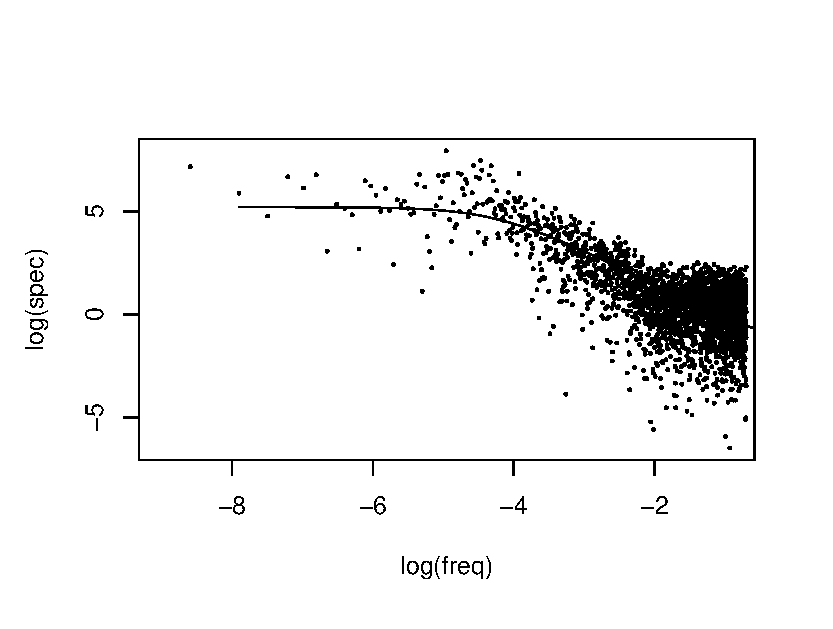
\includegraphics[width=5in]{sb32Whittle.eps}
\caption{Spectral density of water velocity data (circles), along with fitted ARTFIMA spectrum (line).}\label{fig1}
\end{center}
\end{figure}

\begin{example}\label{ExWaterTurb}
Geophysical turbulence in water velocity data (cm/s) was measured in Lake Michigan, Lake Huron, and the Red Cedar River in Michigan, see \cite{Meerschaertsabzikarkumarzeleki} for further details.  Figure \ref{fig1} shows the periodogram and fitted ARTFIMA$(p,d,\lambda,q)$ spectral density function for a data set from Saginaw Bay.  Using the {\tt artfima} package in R and setting $p=q=0$ for a tempered fractional noise, we also set $d=5/6$ (from theory, Kolmogorov scaling, see \cite{Meerschaertsabzikarkumarzeleki} for further details), and this resulted in the parameter fit $\lambda=0.045\ (0.00248)$ using the Whittle estimator, where the second number in parentheses is the standard error.   The plot uses a log-log scale to highlight the power law relation between frequency $\nu$ and spectral density $f_X(\nu)$ for $\log(\nu)>-4$.  The tempering causes a deviation from that line at the lowest frequencies, a feature also seen in the data.  Without fixing $d$, the Whittle estimates are $\lambda=  0.027\ (.00229)$ and $d=0.752\ (.00582)$.  The ARTFIMA model is stationary, and there is ample reason to consider the time series of velocity data as stationary.
\end{example}

\begin{figure}[h]%
\begin{center}
\vskip-50pt
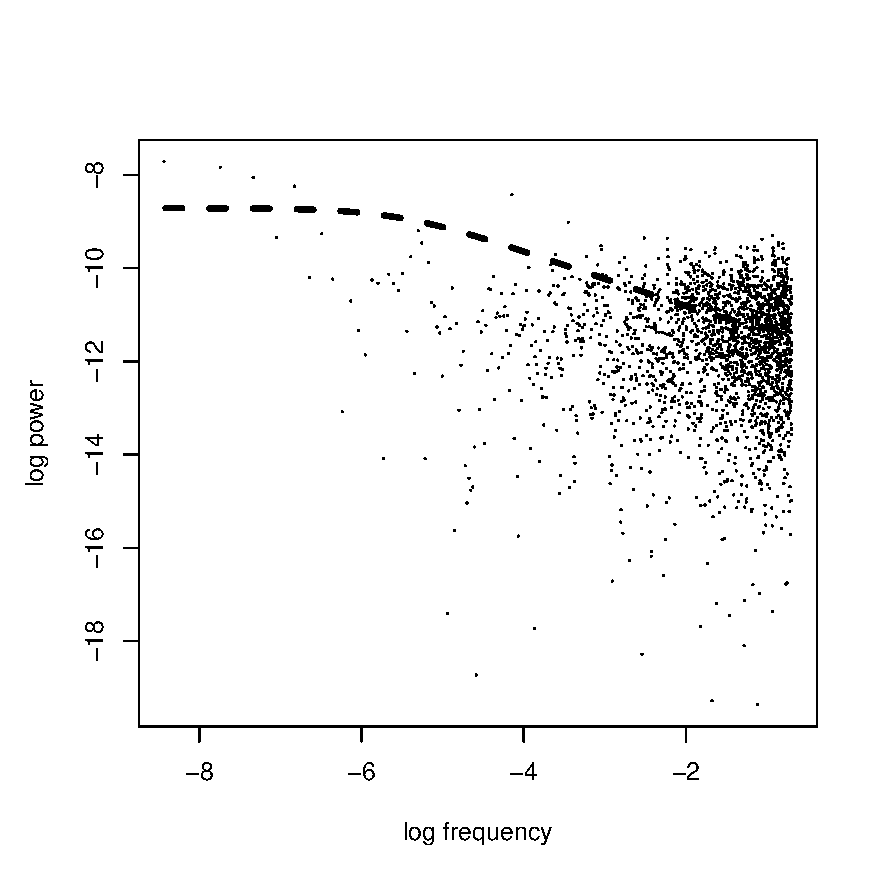
\includegraphics[width=5in]{AMZNspec.eps}
\caption{Spectral density of squared log returns for AMZN stock (circles), along with fitted ARTFIMA spectrum (line).}\label{fig2}
\end{center}
\end{figure}

\begin{example}\label{ExAMZN}
The adjusted closing price $C_t$ for AMZN stock from 1/3/2000 to 12/19/2017 ($n=4520$) was used to compute log returns $R_t=\ln (C_t/C_{t-1})$, which appear uncorrelated.  However, the squared log returns $X_t=R_t^2$ exhibit strong dependence, with an autocorrelation function that remains positive and statistically significant for more than 35 lags.  An ARTFIMA model with $p=q=0$ was fit using the {\tt artfima} package.  The fitted parameters are $d=0.3$ and $\lambda=0.025$.   Figure \ref{fig2} shows that the resulting model spectral density provides a reasonable fit to the periodogram, which follows a power law at moderate frequencies, but levels off at low frequencies.
\end{example}

%ARTFIMA(0,0,0), MLE Algorithm: Whittle, optim: L-BFGS-B
%snr = 0.006, sigmaSq = 1.78695616535146e-05
%log-likelihood = 18289.47, AIC = -36570.93, BIC = -36545.27
%              est.    se(est.)
%mean   0.001130145 8.91756e-05
%d      0.299992020          NA
%lambda 0.025000250          NA

\begin{figure}[h]%
\begin{center}
\vskip-50pt
%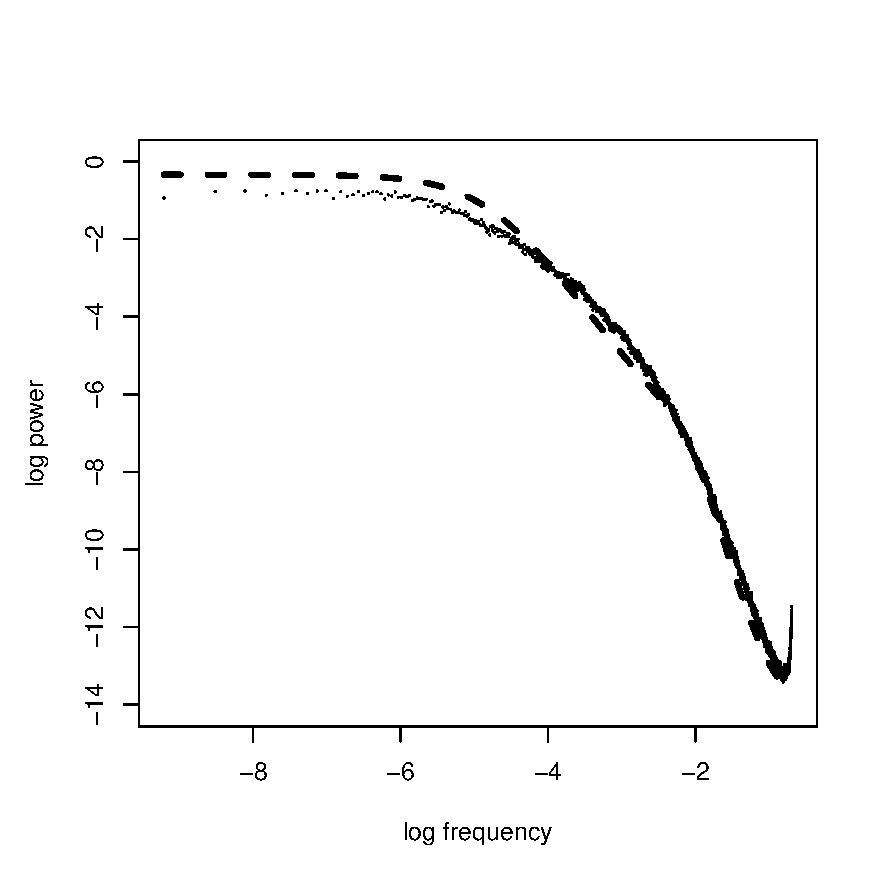
\includegraphics[width=6in]{AvgSpecFit.eps} % fit to first 10,000 then show ave periodogram for 18M
\includegraphics[width=5in]{WelshSpecFit.eps}
\caption{Spectral density of wall turbulence data (circles), along with fitted ARTFIMA spectrum (line).}\label{fig3}
\end{center}
\end{figure}

\begin{example}\label{ExWallTurb}
The vorticity in a turbulent velocity flow near a wall was measured by Morrill-Winter et al. \cite{Wall} at the High
Reynolds Number Boundary Layer Wind Tunnel in Melbourne.  This resulted in a time series with $n=18,000,000$ observations.  We fit an ARTFIMA model with $p=q=0$ to the first 10,000 observations, but the fit was inadequate.  We obtained an adequate fit by including an autoregressive component with $p=2$ and $q=0$.  The fitted parameters were $d=1.34\ (.0486)$, $\lambda=.0531\ (.00646)$, $\phi_1=1.025\ (.0164)$, and $\phi_2=-.0450\ (.01582)$.  The model is causal and invertible. We plot the fitted spectral density against the smoothed periodogram in Figure \ref{fig3}.  Welch's method with a segment length of $L=2000$ was used to smooth the periodogram.  The smoothed periodogram for the entire data set (not shown) is similar. The velocity field in this experiment is designed to be stationary.  With $d=1.34$, the corresponding ARFIMA time series model would have stationary increments.  Hence the ARTFIMA model seems more appropriate.
\end{example}

%ARTFIMA(2,0,0), MLE Algorithm: exact, optim: BFGS
%snr = 306.059, sigmaSq = 4.68879769956692e-05
%log-likelihood = 35645.62, AIC = -71279.24, BIC = -71235.98
%              est.    se(est.)
%mean   -0.01371198 0.001696857
%d       1.33538896 0.048606826
%lambda  0.05307105 0.006463144
%phi(1)  1.02572822 0.016379699
%phi(2) -0.44971282 0.015817899

\begin{figure}[h]%
\begin{center}
\vskip-50pt
\includegraphics[width=5in]{LnKspec.eps}
\caption{Spectral density of hydraulic conductivity data (circles), along with fitted ARTFIMA spectrum (line).}\label{fig4}
\end{center}
\end{figure}

\begin{example}\label{ExKfield}
In Hydrology, the hydraulic conductivity is measured in the field, and used to parameterize contaminant transport models.  High resolution (1.5 cm) hydraulic conductivity data was measured at the MAcroDispersion Experimental (MADE) site in Mississippi by Liu et al.\ \cite{liu2009new}.  We fit the data from one vertical borehole (A121108) using the {\tt artfima} package.   The fitted parameters are $d=1.01\ (.0245)$ and $\lambda=0.00593\ (.00332)$.  The resulting model spectral density and periodogram are plotted in Figure \ref{fig4}.  Note that the fitted spectral density is almost a straight line.  The same data was fit by Meerschaert et al.\  \cite{Kmodel} to an ARFIMA model with $p=q=0$ and $d$=0.9.  The ARTFIMA model is very close to a simple first difference, with stationary increments, and the ARFIMA model with $d=0.9$ also has stationary increments.   However, the K field should be stationary based on the geology, and hence the ARTFIMA model with $\lambda>0$ is preferred, as it provides a stationary time series model.
\end{example}

%ARTFIMA(0,0,0), MLE Algorithm: Whittle, optim: BFGS
%snr = 107.349, sigmaSq = 0.0533836746740295
%log-likelihood = 23.6, AIC = -39.2, BIC = -21.89
%               est.    se(est.)
%mean   -0.944823181 0.141824824
%d       1.019655289 0.024539407
%lambda  0.005932097 0.003317769

\begin{figure}[h]%
\begin{center}
\vskip-50pt
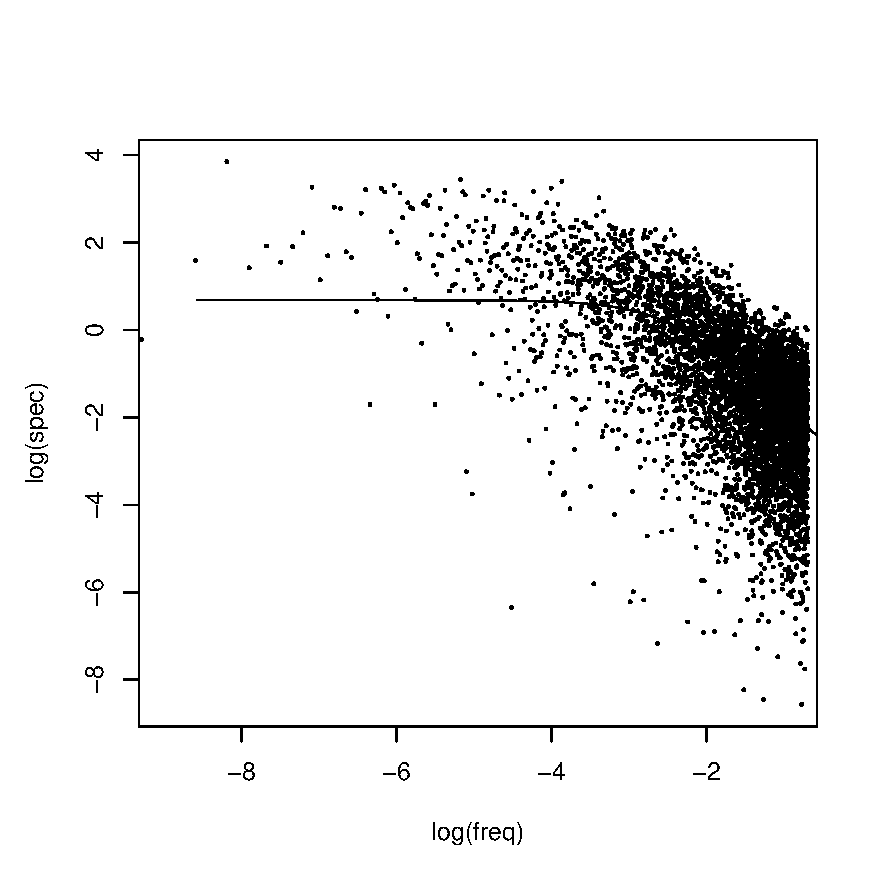
\includegraphics[width=5in]{y1ARTFIMAspec.eps}
\caption{Spectral density of NARCCAP data climate data (circles), along with fitted ARTFIMA spectrum (line).}\label{fig5}
\end{center}
\end{figure}

\begin{example}\label{ExNARCCAP}
A North American Regional Climate Change Assessment Program (NARCCAP) climate model was used to generate 29 years of daily maximum temperature data at 16,100 spatial locations in North America.  The data is freely available at {\tt www.narccap.ucar.edu}.  We examine this data at one location, with sample size $n=10,585$.  The time series shows no evidence of a trend at this location, but significant mean variation and heteroscedasticity with respect to the season.  Hence we subtract the seasonal mean, and divide by the seasonal standard deviation.  We fit an ARTFIMA model to the standardized time series with $d=0.933$ and $\lambda=0.300$ using the {\tt artfima} package.  The fitted spectral density and the periodogram are shown in Figure \ref{fig5}.  The spectral density levels off at low frequencies, consistent with the periodogram.  An ARFIMA model fits the data with $d=0.95$ (not shown).  As there is no evidence of nonstationarity in the standardized time series, the stationary ARTFIMA model seems preferable to the ARFIMA model with $d=0.95$, since the latter has stationary increments.
\end{example}

%ARTFIMA(0,0,0), MLE Algorithm: Whittle, optim: BFGS
%snr = NA, sigmaSq = NA
%log-likelihood = NA, AIC = NA, BIC = NA
%                est.   se(est.)
%mean   -0.0001495601 0.01350665
%d       0.9327859976         NA
%lambda  0.2995577444         NA





\section{Appendix}

{\it Proof of Theorem \ref{th2.3}:}
By inverting the operator $\Delta^{d,\lambda}$, we get
\begin{equation}\label{eq:Xjdefinition}
W_t=\Delta^{-d,\lambda} Z_{t}=\sum_{j=0}^{\infty}(-1)^j e^{-\lambda j}\binom{-d}{j}Z_{t-j}=\sum_{j=0}^{\infty}\omega^{-d,\lambda}_{j}Z_{t-j}.
\end{equation}
Since $\omega^{d,\lambda}_{j}$ has the same sign for all large $j$ (e.g., see \cite[Eq.\ (2.4)]{FCbook}) and
\begin{equation*}
\sum_{j=0}^{\infty}\omega^{d,\lambda}_{j}=\sum_{j=0}^{\infty}(-1)^j e^{-\lambda j}\binom{d}{j}=(1-e^{-\lambda})^{d}<\infty,
\end{equation*}
by the fractional binomial formula (e.g., see Hille \cite[p.\ 147]{Hille1959}) it follows that
\begin{equation}\label{eq:wjabssum}
\sum_{j=0}^{\infty}\big|\omega^{d,\lambda}_{j}\big|<\infty
\end{equation}
for all $\lambda>0$ and all $d\notin{\mathbb Z}$.
Define $A_{\lambda}{B}:=\Delta^{-d,\lambda}\ \Theta(B){\Phi(B)}^{-1}$ and write ${\Theta(z)}{\Phi(z)}^{-1}=\sum_{j=0}^{\infty}b_{j}z^{j}$ for $|z|\leq 1$. Then
\begin{equation*}
A_{\lambda}(z)=(1-e^{-\lambda}z)^{-d}\ {\Theta(z)}{\Phi(z)}^{-1}=\Big(\sum_{i=0}^{\infty}\omega^{-d,\lambda}_{i}z^{i}\Big)
\Big(\sum_{s=0}^{\infty}b_{s}z^{s}\Big)=\sum_{j=0}^{\infty}a^{-d,\lambda}_{j}z^{j},
\end{equation*}
where
\begin{equation}\label{qe:aj defn}
a^{-d,\lambda}_{j}=\sum_{s=0}^{j}\omega^{-d,\lambda}_{s}b_{j-s}
\end{equation}
for $j\geq 0$.
Since $X_t$ satisfies \eqref{eq:artfima general definition}, we can write
\begin{equation}\label{eq:artfima causal}
\begin{split}
X_t&=\Delta^{-d,\lambda}\frac{\Theta(B)}{\Phi(B)}Z_{t}=\left(\sum_{j=0}^{\infty}a^{-d,\lambda}_{j}B^{j}\right)Z_{t}=\sum_{j=0}^{\infty}a^{-d,\lambda}_{j}Z_{t-j}.
\end{split}
\end{equation}
where $a^{-d,\lambda}_{j}$ is given by \eqref{qe:aj defn}. Under assumption \eqref{eq:assumption a}, $\big|{\Theta(z)}/{\Phi(z)}\big|<\infty$, for $|z|\leq 1+\varepsilon$, and the convergence of the series  ${\Theta(z)}/{\Phi(z)}$ implies that $|b_j|\leq C(1+\varepsilon)^{-j}$ for $j\geq 0$ (e.g., see \cite[Theorem 7.2.3]{koul} or \cite[Theorem 3.1.1]{BrockwellDavisTSTM}). By applying \eqref{qe:aj defn}, we have
\begin{equation}\label{sumaj}
\begin{split}
\sum_{j=0}^{\infty}\big|a^{-d,\lambda}_{j}\big|&=\sum_{j=0}^{\infty}\big|\sum_{s=0}^{j}\omega^{-d,\lambda}_{s}b_{j-s}\big|
\leq\sum_{j=0}^{\infty} \sum_{s=0}^{j}\big|\omega^{-d,\lambda}_{s}|\ |b_{j-s}\big|\\
&=\sum_{s=0}^{\infty} \sum_{j=s}^{\infty}\big|\omega^{-d,\lambda}_{s}|\ |b_{j-s}\big|=\sum_{s=0}^{\infty} \sum_{t=0}^{\infty}\big|\omega^{-d,\lambda}_{s}|\ |b_{t}\big|\\
&\leq C \sum_{s=0}^{\infty}\sum_{t=0}^{\infty}\big|\omega^{-d,\lambda}_{s}\big|(1+\varepsilon)^{-t}=C\sum_{s=0}^{\infty}\big|\omega^{-d,\lambda}_{s}\big|\sum_{t=0}^{\infty}(1+\varepsilon)^{-t}<\infty
\end{split}
\end{equation}
since $\sum_{s=0}^{\infty}\big|\omega^{-d,\lambda}_{s}\big|$ is finite by \eqref{eq:wjabssum} and $\sum_{t=0}^{\infty}(1+\varepsilon)^{-t}<\infty$.
Now it follows from Brockwell and Davis \cite[Proposition 3.1.2]{BrockwellDavisTSTM} that $\{X_t\}$, given by \eqref{eq:artfima causal}, is stationary and converges absolutely with probability one and this proves $(a)$.

The white noise sequence $\{Z_{t}\}$ has spectral representation $Z_{t}=\int_{-\pi}^{\pi}e^{it\nu}\ dW(\nu)$ where $W(\nu)$ is an orthogonal increment process on $(-\pi,\pi)$ with $\mathbb{E}[dW(\nu)]=0$, $\mathbb{E}[|dW(\nu)|^2]={d\nu}/{2\pi}$ and $\mathbb{E}[dW(\nu)dW(\eta)]=0$ for $\nu\neq \eta$ (e.g., see \cite[Chapter 2]{koul}).
%Because $\sum_{j=0}^{\infty}\omega^{-d,\lambda}_{j}e^{-ij\nu}=(1-e^{-(\lambda+i\nu)})^{-d}$,  it follows from \cite[Theorem 2.2.1]{koul} that
%\begin{equation}\label{eq:integral rep X}
%X_{t}=\Delta^{-d,\lambda}Z_{t}=\int_{-\pi}^{\pi}e^{it\nu}\big(1-e^{-(\lambda+i\nu)}\big)^{-d}\ dW(\nu).
%\end{equation}
%According to \eqref{eq:TFdiffDef}, we can write
%\begin{equation}\label{eq:delta X defn}
%\Delta^{d,\lambda}_{1}X_{t}=\sum_{j=0}^{\infty}\omega^{d,\lambda}_{j}X_{t-j},
%\end{equation}
%where we considered $h=1$. Now apply the integral representation of $X_t$, given by \eqref{eq:integral rep X}, to rewrite \eqref{eq:delta X defn} as follows:
%\begin{equation*}
%\begin{split}
%\Delta^{d,\lambda}_{1}X_{t}&=\sum_{j=0}^{\infty}\omega^{d,\lambda}_{j}X_{t-j}\\
%&=\sum_{j=0}^{\infty}\omega^{d,\lambda}_{j}\int_{-\pi}^{\pi}e^{i(t-j)\nu}(1-e^{-(\lambda+i\nu)})^{-d}\ dW(\nu)\\
%&=\int_{-\pi}^{\pi}\Big(\sum_{j=0}^{\infty}\omega^{d,\lambda}_{j}e^{-ij\nu}\Big)e^{it\nu}(1-e^{-(\lambda+i\nu)})^{-d}\ dW(\nu)\\
%&=\int_{-\pi}^{\pi}(1-e^{-(\lambda+i\nu)})^{d}(1-e^{-(\lambda+i\nu)})^{-d}e^{it\nu}\ dW(\nu)\\
%&=Z_{t},
%\end{split}
%\end{equation*}
%where in the fourth equation we used the fact that $\sum_{j=0}^{\infty}\omega^{d,\lambda}_{j}e^{-ij\nu}=(1-e^{-(\lambda+i\nu)})^{d}$.
%By the similar argument in part $(a)$, one can show that $\sum_{j=0}^{\infty}\Big|\omega^{d,\lambda}_{j}\Big|<\infty$ and this proves $(b)$.
%
%Recall that $\{Z_{t}\}$ has spectral representation $Z_{t}=\int_{-\pi}^{\pi}e^{it\nu}\ dW(\nu)$ where $W(\nu)$ is an orthogonal increment process on $(-\pi,\pi)$ (see \cite{koul}, Chapter 2).
Because
$\sum_{j=0}^{\infty}a^{-d,\lambda}_{j}e^{-ij\nu}=(1-e^{-(\lambda+i\nu)})^{-d}{\Theta(e^{-i\nu})}/{\Phi(e^{-i\nu})}$,  \cite[Theorem 2.2.1]{koul} implies that
\begin{equation}\label{eq:Xj inverible proof}
X_{t}=\int_{-\pi}^{\pi}e^{it\nu}(1-e^{-(\lambda+i\nu)})^{-d}\ \frac{\Theta(e^{-i\nu})}{\Phi(e^{-i\nu})} dW(\nu).
\end{equation}
Define $B_{\lambda}(B):=\Delta^{d,\lambda}\ {\Phi(B)}/{\Theta(B)}$. Write ${\Phi(z)}/{\Theta(z)}=\sum_{j=0}^{\infty}c_{j}z^{j}$ for $|z|\leq 1$ so that
\begin{equation*}
B_{\lambda}(z)=(1-e^{-\lambda}z)^{d}\ \frac{\Phi(z)}{\Theta(z)}=\Big(\sum_{i=0}^{\infty}\omega^{d,\lambda}_{i}z^{i}\Big)
\Big(\sum_{s=0}^{\infty}c_{s}z^{s}\Big)=\sum_{j=0}^{\infty}c^{d,\lambda}_{j}z^{j},
\end{equation*}
where
\begin{equation}\label{eq:calphaj defn}
c^{d,\lambda}_{j}=\sum_{s=0}^{j}\omega^{d,\lambda}_{s}c_{j-s}
\end{equation}
%\begin{equation}\label{qe:cj defn}
%c^{d,\lambda}_{j}=\sum_{s=0}^{j}\omega^{d,\lambda}_{s}c_{j-s}
%\end{equation}
for $j\geq 0$. It is easy to check that $\sum_{j=0}^{\infty}c^{d,\lambda}_{j}e^{-ij\nu}=(1-e^{-(\lambda+i\nu)})^{d}\ {\Phi(e^{-i\nu})}/{\Theta(e^{-i\nu})}$. Now, apply \eqref{eq:Xj inverible proof} to get:
\begin{equation}\label{eq:artfima general invertible}
\begin{split}
\sum_{j=0}^{\infty}c^{d,\lambda}_{j}B^{j}X_{t}&=\sum_{j=0}^{\infty}c^{d,\lambda}_{j}X_{t-j}\\
&=\sum_{j=0}^{\infty}c^{d,\lambda}_{j}\int_{-\pi}^{\pi}e^{i(t-j)\nu}(1-e^{-(\lambda+i\nu)})^{-d}\frac{\Theta(e^{-i\nu})}{\Phi(e^{-i\nu})}       dW(\nu)\\
&=\int_{-\pi}^{\pi}\Big(\sum_{j=0}^{\infty}c^{d,\lambda}_{j}e^{-ij\nu}\Big)e^{it\nu}(1-e^{-(\lambda+i\nu)})^{-d}
\frac{\Theta(e^{-i\nu})}{\Phi(e^{-i\nu})}\ dW(\nu)\\
&=\int_{-\pi}^{\pi}(1-e^{-(\lambda+i\nu)})^{d}(1-e^{-(\lambda+i\nu)})^{-d}\frac{\Phi(e^{-i\nu})}{\Theta(e^{-i\nu})}
\frac{\Theta(e^{-i\nu})}{\Phi(e^{-i\nu})}e^{it\nu}\ dW(\nu)\\
&=Z_{t}.
\end{split}
\end{equation}
Under assumption \eqref{eq:assumption a}, $\big|{\Phi(z)}/{\Theta(z)}\big|<\infty$, for $|z|\leq 1+\varepsilon$, and the convergence of the series  ${\Phi(z)}/{\Theta(z)}$ implies that
\begin{equation}\label{eq:cj upperbound}
|c_j|\leq K(1+\varepsilon)^{-j},
\end{equation}
for $j\geq 0$, see \cite[Theorem 7.2.3]{koul}. Now apply \eqref{eq:calphaj defn} and \eqref{eq:cj upperbound} to write
\begin{equation*}
\begin{split}
\sum_{j=0}^{\infty}\big|c^{d,\lambda}_{j}\big|&=\sum_{j=0}^{\infty}\big|\sum_{s=0}^{j}\omega^{d,\lambda}_{s}c_{j-s}\big|
\leq\sum_{j=0}^{\infty} \sum_{s=0}^{j}\big|\omega^{d,\lambda}_{s}|\ |c_{j-s}\big|=\sum_{s=0}^{\infty} \sum_{j=s}^{\infty}\big|\omega^{d,\lambda}_{s}|\ |c_{j-s}\big|\\
&=\sum_{s=0}^{\infty} \sum_{t=0}^{\infty}\big|\omega^{d,\lambda}_{s}|\ |c_{t}\big|\leq K \sum_{s=0}^{\infty}\sum_{t=0}^{\infty}\big|\omega^{d,\lambda}_{s}\big|(1+\varepsilon)^{-t}\\
&=K\sum_{s=0}^{\infty}\big|\omega^{d,\lambda}_{s}\big|\sum_{t=0}^{\infty}(1+\varepsilon)^{-t}<\infty
\end{split}
\end{equation*}
since $\sum_{s=0}^{\infty}\big|\omega^{d,\lambda}_{s}\big|$ is finite by \eqref{eq:wjabssum} and $\sum_{t=0}^{\infty}(1+\varepsilon)^{-t}<\infty$.
Now \cite[Proposition 3.1.2]{BrockwellDavisTSTM} implies that $\{Z_t\}$ in \eqref{eq:artfima general invertible} is stationary and converges absolutely with probability one, so $X_{t}$ is invertible, which proves $(b)$.
\hfill $\Box$


{\it Proof of Theorem \ref{thm:Proprties}:  }
(a) Use \eqref{eq:artfima general definition} to write $X_t=\psi_X(B)Z_t$ where $\psi_X(z)=(1-e^{-\lambda}z)^{-d}\Theta(z)/\Phi(z)$. Then the general theory of linear filters implies that $X_t$ has spectral density $f_X(\nu)=|\psi_X(e^{-i\nu})|^2f_Z(\nu)$ using the complex absolute value (e.g., see  \cite{BrockwellDavisTSTM}). Since the white noise process $\{Z_t\}$ has spectral density $f_Z(\nu)=(2\pi)^{-1}\sigma^2$, it follows that \eqref{eq:spectraldensity} holds.

(b) Using \eqref{eq:hUk}, we can rewrite
the spectral density of $X_{t}$ in the form
\begin{equation}\label{eq:spectral artfima general 1}
\begin{split}
f_{X}(\nu)&=\Big(1-e^{-(\lambda+i\nu)}\Big)^{-d}\Big(1-e^{-(\lambda-i\nu)}\Big)^{-d}h_{U}(\nu)\\
&=\frac{\sigma^2}{2\pi}\frac{\Big|\Theta(\omega)\Big|^2}{\Big|\Phi(\omega)\Big|^2}\Big(1-e^{-(\lambda+i\nu)}\Big)^{-d}\Big(1-e^{-(\lambda-i\nu)}\Big)^{-d}\\
&=\frac{\sigma^2}{2\pi}\sum_{l=-q}^{q}\sum_{j=1}^{p}\psi(l)\zeta_{j}\Big[\frac{{\rho_j}^{2p}}{(1-\rho_j\omega)}-\frac{1}{(1-\rho_j^{-1}\omega)}\Big]\\
&\quad\quad\Big(1-e^{-(\lambda+i\nu)}\Big)^{-d}\Big(1-e^{-(\lambda-i\nu)}\Big)^{-d}\omega^{p+l}.
\end{split}
\end{equation}

Next, we compute the covariance function of $X_t$. Recall that the covariance function $\gamma(k)$ and spectral density $f(\nu)$ are connected via $\gamma(k)={\mathbb E}[X_tX_{t+k}]=\int_{-\pi}^{\pi}f(\nu)e^{i\nu k}\ d\nu$. Therefore we have
\begin{equation*}
\begin{split}
\gamma_X(k)&=\int_{-\pi}^{\pi}f_{X}(\nu)e^{i\nu k}\ d\nu\\
&=\frac{\sigma^2}{2\pi}\int_{-\pi}^{\pi}\Bigg[\sum_{l=-q}^{q}\sum_{j=1}^{p}\psi(l)\zeta_{j}\Big[\frac{{\rho_j}^{2p}}{(1-\rho_j\omega)}-\frac{1}{(1-\rho_j^{-1}\omega)}\Big]\\
&\quad\quad\quad\Big(1-e^{-(\lambda+i\nu)}\Big)^{-d}\Big(1-e^{-(\lambda-i\nu)}\Big)^{-d}\omega^{p+l}\Bigg]e^{i\nu k}\ d\nu\\
&=\frac{\sigma^2}{2\pi}\sum_{l=-q}^{q}\sum_{j=1}^{p}\psi(l)\zeta_{j}C(d,\lambda,s-l-p,\rho_j),
\end{split}
\end{equation*}
where
\begin{equation}\label{eq:C lambda definition}
\begin{split}
C(d,\lambda,h,\rho)&=\int_{-\pi}^{\pi}\Big[\frac{{\rho}^{2p}}{(1-\rho\omega)}-\frac{1}{(1-\rho^{-1}\omega)}\Big]\\
&\quad\quad\quad \Big(1-e^{-(\lambda+i\nu)}\Big)^{-d}\Big(1-e^{-(\lambda-i\nu)}\Big)^{-d}e^{i\nu h}\ d\nu.
\end{split}
\end{equation}

Next we write another form of $C(d,\lambda,h,\rho)$ by using the geometric series expansion:
\begin{equation*}
\frac{{\rho}^{2p}}{(1-\rho\omega)}=\frac{{\rho}^{2p}}{(1-\rho e^{-i\nu})}={\rho}^{2p}\sum_{m=0}^{\infty}(\rho e^{-i\nu})^m
\end{equation*}
and
\begin{equation*}
\frac{-1}{(1-\rho^{-1}\omega)}=\frac{-1}{(1-\rho^{-1}e^{-i\nu})}=-1+\sum_{n=0}^{\infty}(\rho e^{i\nu})^{n}=\sum_{n=1}^{\infty}(\rho e^{i\nu})^{n}.
\end{equation*}
Using the spectral density of the ARTFIMA$(0,d,\lambda,0)$ process $W_t=\Delta^{-d,\lambda}Z_t$ given by
\begin{equation}\label{eq:spectralcalc}
\begin{split}
f_W(\nu)
%&=\frac{\sigma^2}{2\pi}\psi_{\lambda}(e^{i\nu})\psi_{\lambda}(e^{-i\nu})\\ &=\frac{\sigma^2}{2\pi}(1-e^{-\lambda}e^{i\nu})^{-d}(1-e^{-\lambda}e^{-i\nu})^{-d}\\
&=\frac{\sigma^2}{2\pi}\Big|1-e^{-(\lambda+i\nu)}\Big|^{-2d}=\frac{\sigma^2}{2\pi}\left(1-2e^{-\lambda}\cos{\nu}+e^{-2\lambda}\right)^{-d} .
\end{split}
\end{equation}
we can then write
\begin{equation}\label{eq:C lambda definition series}
\begin{split}
&C(d,\lambda,h,\rho)\\
&=\int_{-\pi}^{\pi}{\rho}^{2p}\sum_{m=0}^{\infty}(\rho e^{-i\nu})^m\Big(1-e^{-(\lambda+i\nu)}\Big)^{-d}\Big(1-e^{-(\lambda-i\nu)}\Big)^{-d}e^{i\nu h}\ d\nu\\
&+\int_{-\pi}^{\pi}\sum_{n=1}^{\infty}(\rho e^{i\nu})^n \Big(1-e^{-(\lambda+i\nu)}\Big)^{-d}\Big(1-e^{-(\lambda-i\nu)}\Big)^{-d}e^{i\nu h}\ d\nu\\
&=\rho^{2p}\sum_{m=0}^{\infty}\rho^{m}\int_{-\pi}^{\pi}\frac{2\pi}{\sigma^2}f_W(\nu)e^{i\nu(h-m)}\ d\nu+\sum_{n=1}^{\infty}\rho^{n}\int_{-\pi}^{\pi}\frac{2\pi}{\sigma^2}f_W(\nu)e^{i\nu(h+n)}\ d\nu\\
&=\rho^{2p}\sum_{m=0}^{\infty}\rho^{m}\frac{2\pi}{\sigma^2}\gamma_W(h-m)\ d\nu+\sum_{n=1}^{\infty}\rho^{n}\frac{2\pi}{\sigma^2}\gamma_W(h+n).\\
\end{split}
\end{equation}
Next note that the covariance function of $W_t=\Delta^{-d,\lambda}Z_t$ is given by
\begin{equation}\label{eq:covarianceviaspectral}
\begin{split}
\gamma_W(k) &=\int_{-\pi}^{\pi}\cos{(k\nu)}f_W(\nu)\ d\nu\\
&=\frac{\sigma^2}{2\pi}\int_{-\pi}^{\pi}\frac{\cos{(k\nu)}}{\left(1-2e^{-\lambda}\cos{\nu}+e^{-2\lambda}\right)^{d}}\ d\nu\\
&=\frac{\sigma^2}{2\pi}\int_{0}^{2\pi}\frac{(-1)^{k}\cos{(k\nu')}}{\left(1+2e^{-\lambda}\cos{\nu'}+e^{-2\lambda}\right)^{d}}\ d\nu'\ [\nu':=\nu+\pi]\\
&=\sigma^2\frac{e^{-\lambda k}\Gamma(k+d)}{\Gamma(d)\Gamma(k+1)}\ {_2F_1(d;k+d;k+1;e^{-2\lambda})},
\end{split}
\end{equation}
where we applied the integral formula (see \cite{Gradshteyn}, Eq.\ 9.112):
\begin{equation*}
\frac{1}{2\pi}\int_{0}^{2\pi}\frac{\cos{k\omega}}{\left(1-2z\cos{\omega}+z^2\right)^{d}}\ d\omega
=\frac{z^k \Gamma(d+k)}{\Gamma(d)\Gamma(k+1)}\ {_2F_1(d;k+d;k+1;z^2)} .
\end{equation*}
Substituting \eqref{eq:covarianceviaspectral} into \eqref{eq:C lambda definition series} it follows that
\eqref{eq: C lambda computation definition} holds.

To complete the proof, we need to justify the interchange of the sum and integral in \eqref{eq:C lambda definition series}.  Observe that for any $d\notin{\mathbb Z}$ and any $|\rho|<1$ we have
\begin{equation*}
\begin{split}
&\int_{-\pi}^{\pi}\sum_{s=0}^{\infty}\Big|\rho^{s} \Big(1-e^{-(\lambda+i\nu)}\Big)^{-d}\Big(1-e^{-(\lambda-i\nu)}\Big)^{-d}e^{i\nu h}\Big| d\nu\\
&\leq \int_{-\pi}^{\pi}\sum_{s=0}^{\infty}\Big|\rho \Big|^{s}\Big|\Big(1-e^{-(\lambda+i\nu)}\Big)^{-d}\Big(1-e^{-(\lambda-i\nu)}\Big)^{-d}e^{i\nu h}\Big| d\nu\\
&=\frac{1}{1-|\rho|}\int_{-\pi}^{\pi}\Big|\Big(1-e^{-(\lambda+i\nu)}\Big)^{-d}\Big(1-e^{-(\lambda-i\nu)}\Big)^{-d}e^{i\nu h}\Big| d\nu\\
&=\frac{1}{1-|\rho|}\int_{-\pi}^{\pi}(1-2e^{-\lambda}\cos{\nu}+e^{-2\lambda})^{-d}\ d\nu\\
&=2\pi\gamma_W(0)<\infty,
\end{split}
\end{equation*}
where we applied \eqref{eq:covarianceviaspectral} for $k=0$.   \hfill $\Box$

%{\it Proof of Theorem \ref {thm:interesting property of covariance}:  }
%Recall that the covariance function of the zero mean moving average process $W_t=\sum_{j=0}^{\infty}a_j\ Z_{t-j}$ can be written as
%\begin{equation*}
%\gamma_W(k)=\mathbb{E}[W_0 W_k]=\sigma^2 \sum_{j=0}^{\infty}a_{j}a_{j+k}
%\end{equation*}
%for $k\geq 0$ (see \cite{koul}, Chapter 2). Therefore, using \eqref{eq:Xjdefinition} we can write
%\begin{equation*}
%\gamma_W(k)=\mathbb{E}[W_0 W_k]=\sigma^2 \sum_{j=0}^{\infty}\omega^{-d,\lambda}_{j}\omega^{-d,\lambda}_{j+k}
%\end{equation*}
%for $k\geq 0$. Since $\sum_{j=0}^{\infty}\big|\omega^{-d,\lambda}_{j}\big|<\infty$ and $\sum_{j=0}^{\infty}\omega^{-d,\lambda}_{j}=(1-e^{-\lambda})^{-d}$, it follows that
%\begin{equation*}
%\sum_{k=0}^{+\infty}\big|\gamma_W(k)\big|\leq\sigma^2 \sum_{k=0}^{\infty}\sum_{j=0}^{\infty}\big|\omega^{-d,\lambda}_{j}\omega^{-d,\lambda}_{j+k}\big|
%\leq\sigma^{2}\Big(\sum_{j=0}^{\infty}\Big|\omega^{-d,\lambda}_{j}\Big|\Big)^{2}<\infty
%\end{equation*}
%and
%\begin{equation*}
%\begin{split}
%\sum_{k=-\infty}^{\infty}\gamma_W(k)&=\gamma(0)+2\sum_{k=1}^{\infty}\gamma_W(k)\\
%&=\sigma^{2}\Big(\sum_{j=0}^{\infty}(\omega^{-d,\lambda}_{j})^{2}+2\sum_{k=1}^{\infty}\sum_{j=0}^{\infty}\omega^{-d,\lambda}_{j}\omega^{-d,\lambda}_{j+k}\Big)\\
%&=\sigma^{2}\Big(\sum_{j=0}^{\infty}(\omega^{-d,\lambda}_{j})^{2}+2\sum_{j=0}^{\infty}\sum_{l=j+1}^{\infty}\omega^{-d,\lambda}_{j}\omega^{-d,\lambda}_{l}\Big)\\
%&=\sigma^{2}\Big(\sum_{j=0}^{\infty}(\omega^{-d,\lambda}_{j})^{2}+\sum_{j=0}^{\infty}\sum_{l=0,l\neq j}^{\infty}\omega^{-d,\lambda}_{j}\omega^{-d,\lambda}_{l}\Big)\\
%&=\sigma^{2}\Big(\sum_{j=0}^{\infty}\omega^{-d,\lambda}_{j}\Big)^2=\sigma^{2}(1-e^{-\lambda})^{-2d}
%\end{split}
%\end{equation*}
%and this completes the proof.
%
%\hfill $\Box$


{\it Proof of Theorem \ref{thm:consistency Whittle}}:
First we note that the ARTFIMA$(p,d,\lambda,q)$ time series is ergodic since it is an infinite moving average with ergodic innovations $\{ Z_t\}_{ t\in\mathbb{Z} }$, see \cite[Corollarly 2.1.8]{Samorodnitsky}.
%For this, it is sufficient (e.g., see Hamilton \cite[p.\ 504]{Hamilton}) that
%\begin{equation}\label{ConditionHamilton}
%\sum_{j=0}^{\infty}j|a^{-d,\lambda}_{j}|<\infty
%\end{equation}
%where $a^{-d,\lambda}_{j}$ are the moving average weights defined by \eqref{qe:aj defn}.  As in the proof of Theorem \ref{th2.3} we have  $|b_j|\leq C_1(1+\varepsilon)^{-j}$ for $j\geq 0$.  An application of Stirling's approximation (e.g., see \cite[Eq.\ (2.5)]{FCbook}) yields that $|\omega^{-d,\lambda}_{j}|\leq C_2 j^{\alpha-1}e^{-\lambda j}$ for all $j>0$, and note that $\omega^{-d,\lambda}_{0}=1$.
%%From \eqref{sumaj} it follows that $|a^{-d,\lambda}_{j}|\leq C_3$ for all $j\geq 0$.
%Now write
%\begin{equation*}\begin{split}
%\sum_{j=0}^{\infty}&j|a^{-d_0,\lambda_{0}}_{j}|
%%&= \sum_{j=0}^{\infty}j\left|\sum_{s=0}^{j}\omega^{-d,\lambda}_{s}b_{j-s}\right|\\
%\leq  \sum_{j=0}^{\infty}\sum_{s=0}^{j}j\left|\omega^{-d,\lambda}_{s}b_{j-s}\right|
%= \sum_{s=0}^{\infty}\sum_{j=s}^{\infty}j\left|\omega^{-d,\lambda}_{s}b_{j-s}\right|\\
%%&=  \sum_{s=0}^{\infty}\sum_{t=0}^{\infty}(s+t)\left|\omega^{-d,\lambda}_{s}b_{t}\right|
%&\leq  C_1\sum_{s=0}^{\infty}\sum_{t=0}^{\infty}(s+t)\left|\omega^{-d,\lambda}_{s}\right|(1+\varepsilon)^{-t}:=  C_1\sum_{s=0}^{\infty}\left|\omega^{-d,\lambda}_{s}\right|(A+Bs)\\
%\end{split}\end{equation*}
%where
%\begin{equation*}\begin{split}
%A&=\sum_{t=1}^{\infty}t(1+\varepsilon)^{-t}=(1+\varepsilon)^{-1}(1-(1+\varepsilon)^{-1})^{-2}<\infty ,\\
%B&=\sum_{t=0}^{\infty}(1+\varepsilon)^{-t}=(1-(1+\varepsilon)^{-1})^{-1}<\infty .
%\end{split}\end{equation*}
%Since
%\begin{equation*}\begin{split}
%\sum_{s=0}^{\infty}s\left|\omega^{-d,\lambda}_{s}\right|&\leq \sum_{s=1}^{\infty}C_2 j^{\alpha}e^{-\lambda j}<\infty
%\end{split}\end{equation*}
%it follows using \eqref{eq:wjabssum} that \eqref{ConditionHamilton} holds, and hence the time series is ergodic.
Then we can apply Theorem 8.2.1 in \cite{koul} (see also Theorem 1 in Hannan \cite{hannan}).  This requires us to verify the conditions:
\begin{itemize}
\item[(1)] The parameters $(\sigma,\ttheta)\in\Omega$ determine the spectral density function \eqref{eq:spectral artfima general 1secondfrom} uniquely.
\item[(2)] ${1}/({K(\nu,\ttheta)+a})$ is continuous in $(\nu,\ttheta)\in(-\pi,\pi)\times\Xi$, for all $a>0$.
\item[(3)] $\sum_{j=0}^{\infty}(a^{-d,\lambda}_{j})^{2}<\infty$ and $a^{-d,\lambda}_{0}=1$ where $a^{-d,\lambda}_{j}$ is given by \eqref{qe:aj defn}.
\end{itemize}
Since $d$ is not an integer, it is easy to see that condition (1) holds.  Since $K(\nu,\ttheta)$ is continuous and strictly positive for $\lambda>0$, it is apparent that condition (2) holds.
%By following the proof of Theorem \ref{thm:interesting property of covariance} for the ARTFIMA$(p,d,\lambda,q)$ time series, one can see that
%\begin{equation*}
%\begin{split}
%\sum_{k=-\infty}^{\infty}\gamma_X(k)&=\gamma(0)+2\sum_{k=1}^{\infty}\gamma_X(k)\\
%&=\sigma^{2}\Big(\sum_{j=0}^{\infty}a^{-d,\lambda}_{j}\Big)^2=\sigma^{2}(1-e^{-\lambda})^{-2d}\big({\Theta(z)}/{\Phi(z)}\big)^{2}<\infty
%\end{split}
%\end{equation*}
%which implies that $\sum_{j=0}^{\infty}(a^{-d,\lambda}_{j})^{2}=\gamma_{X}(0)<\infty$.
From \eqref{sumaj} it follows that $|a^{-d,\lambda}_{j}|\leq C_3$ for all $j\geq 0$.  Then by a similar argument to that of \eqref{sumaj} it can be shown that
\begin{equation}\label{Condition3}
\sum_{j=0}^{\infty}j(a^{-d,\lambda}_{j})^2\leq C_3 \sum_{j=0}^{\infty}j|a^{-d,\lambda}_{j}|<\infty .
\end{equation}
It is also easy to see that $a^{-d,\lambda}_{0}=\omega^{-d,\lambda}_{0}b_{0}=1$.  Then Condition (3) follows, and now the proof is complete.
\hfill $\Box$.

\begin{proof}[Proof of Theorem \ref{thm:asymptoticnormality}]
The result follows from Theorem 2 in Hannan \cite{hannan} or Theorem 8.3.1 in Giraitis et al. \cite{koul}, once we verify the following conditions:
\begin{itemize}
%\item $\mathbb{E}(Z_{j}|\mathfrak{F_{j-1}})=0$ and $\mathbb{E}(Z^{2}_{j}|\mathfrak{F_{j-1}})=0$, where $\mathfrak{F_{j}}$ is the Borel field generated by $Z_{i}$ for $i\leq j$, (This condition was considered in Hannan \cite{hannan}, but Giraitis et al. \cite[p. 214]{koul} considered $Z_{j}$ as an i.i.d random variables with zero mean and variance $\sigma^2$ and finite fourth moment).
\item[(1)] $K(\nu,\ttheta)\geq a>0$ for $\nu\in(-\pi,\pi)$.
\item[(2)] $K(\nu,\ttheta)$ is a twice differentiable function of parameters $\lambda,d,\phi_1,\ldots,\phi_p,\theta_1,\ldots,\theta_q$.
\item[(3)] Equation \eqref{Condition3} holds.
\end{itemize}
Property (1) follows from the fact that $|1-e^{-(\lambda+i\nu)}|>1-e^{-\lambda}$ for all $\nu$.  Property (2) is apparent from the first line of \eqref{eq:spectral artfima general 1secondfrom}, since $\lambda>0$. Condition (3) was verified in the proof of Theorem \ref{thm:consistency Whittle}.
\end{proof}


{\it Proof of Theorem \ref{thm:Wdetails} }:
The matrix $\bf I$ is the same as the matrix $\bf W$ in Brockwell and Davis \cite[Theorem 10.8.2, p. 386]{BrockwellDavisTSTM} for the asymptotic covariance of the ARMA$(p,q)$ parameter estimates, see also Box and Jenkins \cite[p.240]{BoxJenkins} or Li and McLeod \cite[Section 3]{LiMcLeod}.  This proves part (1).
%However, for the sake of completeness, we give some details about the matrix $\bf I$.
%According to the argument in \cite[p.386--387]{BrockwellDavisTSTM}, for $1\leq j\leq p$ and $1\leq k\leq p$:
%\begin{equation*}
%w_{j,k}=\frac{1}{4\pi}\int_{-\pi}^{\pi}(e^{-i(j-k)\nu}+e^{i(j-k)\nu})|\Phi(e^{-i\nu})|^{2}\ d\nu
%=\mathbb{E}[M_{t-j+1}M_{t-k+1}]
%\end{equation*}
%where $\{M_t\}$ is the autoregressive process defined by
%\begin{equation}\label{eq:Mprocess}
%\Phi(B)M_{t}=Z_{t}\qquad \{Z_t\}\sim {\text WN}(0,1).
%\end{equation}
%Hence we will write $w_{j,k}=\gamma_{M}(j-k)$.
%
%A same argument shows that for $p+1\leq j\leq p+q$ and $p+1\leq k\leq p+q$
%\begin{equation*}
%w_{j,k}=\frac{1}{4\pi}\int_{-\pi}^{\pi}(e^{-i(j-k)\nu}+e^{i(j-k)\nu})|\Theta(e^{-i\nu})|^{2}\ d\nu
%=\mathbb{E}[N_{t-j+1}N_{t-k+1}]
%\end{equation*}
%where $\{N_t\}$ is the autoregressive process defined by
%\begin{equation}\label{eq:Nprocess}
%\Theta(B)N_{t}=Z_{t}\qquad \{Z_t\}\sim {\text WN}(0,1).
%\end{equation}
%Therefore we will write $w_{j,k}=\gamma_{N}(j-k)$.
%
%Next, assume $1\leq j\leq p$ and $k=p+m\geq p+1$ (and $k\leq p+q$). Then
%\begin{equation*}
%\begin{split}
%w_{j,p+m}&=\frac{1}{4\pi}\int_{-\pi}^{\pi}\frac{\partial{\log K(\nu,\ttheta_0)}}{\partial{\phi_j}}\frac{\partial{\log K(\nu,\ttheta_0)}}{\partial{\ttheta_m}}\ d\nu\\
%&=\frac{1}{4\pi}\int_{-\pi}^{\pi}
%\big[e^{i(m-j)\nu}\Phi^{-1}(e^{-i\nu})\Theta^{-1}(e^{i\nu})+
%e^{-i(m-j)\nu}\Phi^{-1}(e^{i\nu})\Theta^{-1}(e^{-i\nu})\big]\ d\nu.
%\end{split}
%\end{equation*}
%In fact, for $1\leq j\leq p$ and $1\leq m\leq q$, it can be seen (\cite[p.387]{BrockwellDavisTSTM}) that
%\begin{equation*}
%w_{j,p+m}=\mathbb{E}[M_{t-j+1}N_{t-m+1}]
%\end{equation*}
%where $\{M_t\}$ and $\{N_t\}$ are given by \eqref{eq:Mprocess} and \eqref{eq:Nprocess}. By the symmetry of the matrix $\bf I$,
%\begin{equation*}
%w_{p+m,k}=\mathbb{E}[N_{t-m+1}M_{t-k+1}]
%\end{equation*}
%for $1\leq m\leq q$ and $1\leq k\leq p$.
%Based on the above results, one write the matrix $\bf I$ as the following:
%\begin{equation*}
%\begin{pmatrix}
%    \gamma_{M}(0) & \gamma_{M}(1) & \ldots & \gamma_{M}(p-1)& | & \gamma_{MN}(0) & \gamma_{MN}(1) & \ldots & \gamma_{MN}(q-1) \\
%    \gamma_{M}(1) & \gamma_{M}(0) & \ldots & \gamma_{M}(p-2) & | & \gamma_{MN}(-1) & \gamma_{MN}(0) & \ldots & \gamma_{MN}(q-2) \\
%     \vdots       & \vdots & \vdots & \vdots & | & \vdots & \vdots & \vdots & \vdots \\
%    \gamma_{M}(p-1)&\gamma_{M}(p-2) & \ldots & \gamma_{M}(0) & | & \gamma_{MN}(1-p) & \gamma_{MN}(2-p) & \ldots & \gamma_{MN}(q-p) \\
%    -- & -- & -- & -- & | & -- & -- & -- & -- \\
%    \gamma_{NM}(0) & \gamma_{NM}(1) & \ldots & \gamma_{NM}(p-1) & | & \gamma_{N}(0) & \gamma_{N}(1) & \ldots & \gamma_{N}(q-1) \\
%    \gamma_{NM}(-1) & \gamma_{NM}(0) & \ldots & \gamma_{NM}(p-2) & | & \gamma_{N}(-1) & \gamma_{N}(0) & \ldots & \gamma_{N}(q-2) \\
%   \vdots       & \vdots & \vdots & \vdots & | & \vdots & \vdots & \vdots & \vdots \\
%    \gamma_{NM}(1-q) & \gamma_{NM}(2-q) & \ldots & \gamma_{NM}(p-q) &  | & \gamma_{N}(1-q) & \gamma_{N}(2-q) & \ldots & \gamma_{N}(0) \\
%\end{pmatrix}
%\end{equation*}

To prove the remaining parts, write
\begin{equation*}
\log K(\nu,\ttheta)=\log(\big|\Theta(e^{-i\nu}\big)\big|^2)-\log(\big|\Phi(e^{-i\nu})\big|^2)-d\log(1-2e^{-\lambda}\cos{\nu}+e^{-2\lambda}).
\end{equation*}
Observe that
\begin{equation*}
\begin{split}
\log(\big|\Phi(e^{-i\nu}\big)\big|^2)&=\log(\Phi(e^{-i\nu}))+\log(\Phi(e^{i\nu}))\\
&=\log(1+\phi_{1}e^{-i\nu}+\ldots+\phi_{j}e^{-i\nu j}+\ldots+\phi_{p}e^{-i\nu p})\\
&+\log(1+\phi_{1}e^{i\nu}+\ldots+\phi_{j}e^{i\nu j}+\ldots+\phi_{p}e^{i\nu p})
\end{split}
\end{equation*}
and then
\begin{equation}\label{eq:derivativesphi}
\begin{split}
\frac{\partial{\log K(\nu,\ttheta_0)}}{\partial{\phi_j}}&=\frac{\partial{\log(\big|\Phi(e^{-i\nu}\big)\big|^2)}}{\partial{\phi_j}}
=\frac{\partial}{\partial{\phi_j}}\big\{\log(\Phi(e^{-i\nu}))+\log(\Phi(e^{i\nu}))\big\}\\
&=\frac{\partial}{\partial{\phi_j}}\log(1+\phi_{1}e^{-i\nu}+\ldots+\phi_{j}e^{-i\nu j}+\ldots+\phi_{p}e^{-i\nu p})\\
&+\frac{\partial}{\partial{\phi_j}}\log(1+\phi_{1}e^{i\nu}+\ldots+\phi_{j}e^{i\nu j}+\ldots+\phi_{p}e^{i\nu p})\\
&=\frac{e^{-i\nu j}}{1+\phi_{1}e^{-i\nu}+\ldots+\phi_{j}e^{-i\nu j}+\ldots+\phi_{p}e^{-i\nu p}}\\
&+\frac{e^{i\nu j}}{1+\phi_{1}e^{i\nu}+\ldots+\phi_{j}e^{i\nu j}+\ldots+\phi_{p}e^{i\nu p}}\\
&=e^{-i\nu j}\Phi^{-1}(e^{-i\nu})+e^{i\nu j}\Phi^{-1}(e^{i\nu}).
\end{split}
\end{equation}
By a similar argument,
\begin{equation*}
\begin{split}
\log(\big|\Theta(e^{-i\nu}\big)\big|^2)&=\log(\Theta(e^{-i\nu}))+\log(\Theta(e^{i\nu}))\\
&=\log(1+\theta_{1}e^{-i\nu}+\ldots+\theta_{j}e^{-i\nu j}+\ldots+\theta_{q}e^{-i\nu q})\\
&+\log(1+\theta_{1}e^{i\nu}+\ldots+\theta_{j}e^{i\nu j}+\ldots+\theta_{q}e^{i\nu q})
\end{split}
\end{equation*}
and consequently
\begin{equation}\label{eq:derivativestheta}
\begin{split}
\frac{\partial{\log K(\nu,\ttheta_0)}}{\partial{\theta_j}}&=\frac{\partial{\log(\big|\Theta(e^{-i\nu}\big)\big|^2)}}{\partial{\theta_j}}
=\frac{\partial}{\partial{\theta_j}}\big\{\log(\Theta(e^{-i\nu}))+\log(\Theta(e^{i\nu}))\big\}\\
&=\frac{\partial}{\partial{\theta_j}}\log(1+\theta_{1}e^{-i\nu}+\ldots+\theta_{j}e^{-i\nu j}+\ldots+\theta_{q}e^{-i\nu q})\\
&+\frac{\partial}{\partial{\theta_j}}\log(1+\theta_{1}e^{i\nu}+\ldots+\theta_{j}e^{i\nu j}+\ldots+\theta_{q}e^{i\nu q})\\
&=\frac{e^{-i\nu j}}{1+\theta_{1}e^{-i\nu}+\ldots+\theta_{j}e^{-i\nu j}+\ldots+\theta_{q}e^{-i\nu q}}\\
&+\frac{e^{i\nu j}}{1+\theta_{1}e^{i\nu}+\ldots+\theta_{j}e^{i\nu j}+\ldots+\theta_{q}e^{i\nu q}}\\
&=e^{-i\nu j}\Theta^{-1}(e^{-i\nu})+e^{i\nu j}\Theta^{-1}(e^{i\nu}).
\end{split}
\end{equation}
It is also easy to see that
\begin{equation}\label{eq:derivatived}
\frac{\partial{\log K(\nu,\ttheta_0)}}{\partial{d}}=-\log(1-2e^{-\lambda}\cos{\nu}+e^{-2\lambda})
\end{equation}
and
\begin{equation}\label{eq:derivativelambda}
\frac{\partial{\log K(\nu,\ttheta_0)}}{\partial{\lambda}}=-2d e^{-\lambda}\Big(\frac{\cos{\nu}-e^{-\lambda}}{1-2e^{-\lambda}\cos{\nu}+e^{-2\lambda}}\Big)
\end{equation}

Then part (2) follows easily.

As for (3), the formula for $v_{1,1}$ follows immediately from \eqref{eq:derivatived}.  A useful approximation will be provided in a remark following the proof.  Next write
\begin{equation}\label{eq:v22spectraldensityintegral1}
\begin{split}
v_{2,2}
%&=\frac{1}{4\pi}\int_{-\pi}^{\pi}\Big(\frac{\partial{\log K(\nu,\ttheta_0)}}{\partial{\lambda}}\Big)^{2} d\nu\\
&=\frac{1}{4\pi}\int_{-\pi}^{\pi}\Big(-2d e^{-\lambda}\Big(\frac{\cos{\nu}-e^{-\lambda}}{1-2e^{-\lambda}\cos{\nu}+e^{-2\lambda}}\Big)\Big)^{2}\ d\nu\\
&=\frac{{d}^{2}}{4\pi}
\int_{-\pi}^{\pi}\Big(1+\frac{e^{-2\lambda}-1}{1-2e^{-\lambda}\cos{\nu}+e^{-2\lambda}}\Big)^{2}d\nu\\
&=\frac{d^2}{4\pi}\int_{-\pi}^{\pi}\Big[1+\frac{(e^{-2\lambda}-1)^{2}}{(1+e^{-2\lambda}-2e^{-\lambda}\cos{\nu})^{2}}+\frac{2(e^{-2\lambda}-1)}{1+e^{-2\lambda}-2e^{-\lambda}\cos{\nu}}\Big]d\nu.
\end{split}
\end{equation}
Observe that
\begin{equation}\label{eq:v22spectraldensityintegral2}
\begin{split}
\int_{-\pi}^{\pi}\frac{d\nu}{(1+e^{-2\lambda}-2e^{-\lambda}\cos{\nu})^{2}}&=2\int_{0}^{\pi}\frac{d\nu}{(1+e^{-2\lambda}-2e^{-\lambda}\cos{\nu})^{2}}\\
&=\frac{2\pi(1+e^{-2\lambda})}{(1-e^{-2\lambda})^{3}}
\end{split}
\end{equation}
where we used the standard formula
\begin{equation}\label{eq:standardformula1}
\int_{0}^{\pi}\frac{d\nu}{(1+a^{2}-2a\cos{\nu})^{n}}=\frac{\pi}{(1-a^2)^{n}}\sum_{k=0}^{n-1}\frac{(n+k-1)!}{(k!)^{2}(n-k-1)!}\big(\frac{a^2}{1-a^{2}}\big)^{k}
\end{equation}
for $a^{2}<1$ (see \cite[p. 608]{Gradshteyn}).
By applying \eqref{eq:standardformula1} for $n=1$, we also have
\begin{equation}\label{eq:v22spectraldensityintegral3}
\int_{-\pi}^{\pi}\frac{d\nu}{(1+e^{-2\lambda}-2e^{-\lambda}\cos{\nu})}=\frac{2\pi}{1-e^{-2\lambda}}.
\end{equation}
%since
%\begin{equation*}
%\int_{-\pi}^{\pi}\frac{d\nu}{(1+a^{2}-2a\cos{\nu})}=\frac{2\pi}{1-a^{2}}
%\end{equation*}
%for $a^{2}<1$ (see \cite[p.696]{Gradshteyn}).
%since $X_{2}$ is $\rm ARTFIMA(0,\lambda,1,0)$.
Therefore, from \eqref{eq:v22spectraldensityintegral1}, \eqref{eq:v22spectraldensityintegral2} and \eqref{eq:v22spectraldensityintegral3}:
\begin{equation}\label{eq:v22spectraldensityintegral4}
\begin{split}
v_{2,2}
%&=\frac{1}{4\pi}\int_{-\pi}^{\pi}\Big(\frac{\partial{\log K(\nu,\ttheta_0)}}{\partial{\lambda}}\Big)^{2}\ d\nu
=\frac{d^2}{4\pi}
\Big[2\pi+\frac{2\pi(1+e^{-2\lambda})}{(1-e^{-2\lambda})}-4\pi\Big]=\frac{d^2 e^{-2\lambda}}{1-e^{-2\lambda}}
\end{split}
\end{equation}
as claimed.
Finally, write
\begin{equation}\label{eq:v1v2calculation}
\begin{split}
v_{1,2}=v_{2,1}
%&=\frac{1}{4\pi}\int_{-\pi}^{\pi}\frac{\partial{\log K(\nu,\ttheta_0)}}{\partial{d}}\frac{\partial{\log K(\nu,\ttheta_0)}}{\partial{\lambda}} d\nu\\
&=\frac{-d}{4\pi}\int_{-\pi}^{\pi}\big(\log(1-2e^{-\lambda}\cos{\nu}+e^{-2\lambda})\big)
\Big(1+\frac{e^{-2\lambda}-1}{1-2e^{-\lambda}\cos{\nu}+e^{-2\lambda}}\Big)\ d\nu\\
&=\frac{-d}{4\pi}(I_{1}+I_{2})
\end{split}\end{equation}
where
\begin{equation*}\begin{split}
I_{1}&:=\int_{-\pi}^{\pi}\ln(1-2e^{-\lambda}\cos{\nu}+e^{-2\lambda})\ d\nu\\
I_{2}&:=\int_{-\pi}^{\pi}\frac{(e^{-2\lambda}-1)\ln(1-2e^{-\lambda}\cos{\nu}+e^{-2\lambda})}{1-2e^{-\lambda}\cos{\nu}+e^{-2\lambda}}\ d\nu.
\end{split}\end{equation*}
To calculate $I_{1}$, use integration by parts to write
\begin{equation}\label{eq:I1calculation2}
\begin{split}
I_{1}&=\nu\ln(1-2e^{-\lambda}\cos{\nu}+e^{-2\lambda})\big]^{\pi}_{-\pi}
-\int_{-\pi}^{\pi}\frac{2e^{-\lambda}\nu \sin{\nu}}{1-2e^{-\lambda}\cos{\nu}+e^{-2\lambda}}\ d\nu\\
&=2\pi\ln(1+e^{-\lambda})^{2}-4e^{-\lambda}\int_{0}^{\pi}\frac{\nu \sin{\nu}}{1-2e^{-\lambda}\cos{\nu}+e^{-2\lambda}}\ d\nu\\
&=4\pi\ln(1+e^{-\lambda})-4\pi\ln(1+e^{-\lambda})=0,
\end{split}
\end{equation}
since
\begin{equation*}
\int_{0}^{\pi}\frac{\nu \sin{\nu}}{1-2a\cos{\nu}+a^{2}}\ d\nu=\frac{\pi}{a}\ln(1+a)
\end{equation*}
for $a^2<1$ and $a\neq 0$ (see \cite[No 4, p. 696]{Gradshteyn}).
%
%
%To calculate $I_{1}$, given by \eqref{eq:I1definition}, one can use the fact that
%\begin{equation*}
%\ln\ x=(x-1)-\frac{(x-1)^2}{2}+\frac{(x-1)^3}{3}-\frac{(x-1)^4}{4}+\ldots ,
%\end{equation*}
%for $0<x\leq 2$. Therefore
%\begin{equation*}
%\ln(1-2e^{-\lambda}\cos{\nu}+e^{-2\lambda})\approx -2e^{-\lambda\cos{\nu}}+e^{-2\lambda}
%\end{equation*}
%and then
%\begin{equation}\label{eq:I1calculation}
%\begin{split}
%I_{1}&=\int_{-\pi}^{\pi}\ln(1-2e^{-\lambda}\cos{\nu}+e^{-2\lambda})\ d\nu\approx\int_{-\pi}^{\pi}-2e^{-\lambda}\cos{\nu}+e^{-2\lambda}\ d\nu\\
%&=2\pi\ e^{-2\lambda}
%\end{split}
%\end{equation}
%(Farzad: I got the idea for calculation $I_{1}$ from \cite{lateron}).

In order to calculate $I_{2}$, we use the standard formula
\begin{equation*}
\int_{0}^{\pi}\frac{\ln(1-2a\cos{\nu}+a^{2})}{1-2b\cos{\nu}+b^{2}}\ d\nu=\frac{2\pi\ln(1-ab)}{1-b^{2}}
\end{equation*}
for $a^{2}\leq 1$ and $b^{2}<1$ (see \cite[No. 16, p. 925]{Gradshteyn}). In our case $a=b=e^{-\lambda}$. Therefore
\begin{equation}\label{eq:I2calculation}
\begin{split}
I_{2}&=(e^{-2\lambda}-1)\int_{-\pi}^{\pi}\frac{\ln(1-2e^{-\lambda}\cos{\nu}+e^{-2\lambda})}{1-2e^{-\lambda}\cos{\nu}+e^{-2\lambda}}\ d\nu\\
&=2(e^{-2\lambda}-1)\int_{0}^{\pi}\frac{\ln(1-2e^{-\lambda}\cos{\nu}+e^{-2\lambda})}{1-2e^{-\lambda}\cos{\nu}+e^{-2\lambda}}\ d\nu\\
&=\frac{4\pi\ln(1-e^{-2\lambda})}{1-e^{-2\lambda}}(e^{-2\lambda}-1)=-4\pi\ln(1-e^{-2\lambda}).
\end{split}
\end{equation}
Now, from \eqref{eq:v1v2calculation}, \eqref{eq:I1calculation2} and \eqref{eq:I2calculation}, we have
\begin{equation}
v_{1,2}=v_{2,1}=\frac{-d}{4\pi}\big[-4\pi\ln(1-e^{-2\lambda})\big]=d\ln(1-e^{-2\lambda}),
\end{equation}
and this completes the proof of (3).
\hfill $\Box$

\begin{proof}[Proof of Theorem \ref{th3.6}]
The proof follows from Theorem 1 in \cite{hannan}.
\end{proof}

\begin{proof}[Proof of Theorem \ref{th3.7}]
This follows immediately from Theorem \ref{thm:asymptoticnormality}, Theorem \ref{thm:Wdetails}, and Theorem 10.8.2 in Brockwell and Davis \cite{BrockwellDavisTSTM}.
\end{proof}



\section{Acknowledgments}
We would like to thank Mantha Phanikumar, Michigan State University, for access to the water velocity data, and Joe Klewicki, University of Delaware, for the wall turbulence data, as well as helpful discussions.

\begin{thebibliography}{1}

%\bibitem{abramowitz}
%M. Abramowitz and I. Stegun  (1965)  Handbook of mathematical functions, ninth edition, Dover, New York.
%\bibitem{BartonVincent}
%R. J. ~Barton and H. ~Vincent Poor.
%\newblock{\em  Signal Detection in Fractional Gaussian Noise,
%IEEE trans}. on information theory 34 (1988), no. 5, 943u959.

%\bibitem{Barton}
%R.J. ~Barton.
%\newblock{\em signal detection fractional Gaussian noise and an RKHS approach to robust detection and estimation}

%\bibitem{BaiTaqqu}
%Bai, S., Taqqu, M.,S. (2014). Generalized Hermite processes, discrete chaos and limit theorems. Stochastic processes and their applications
%{\bf 124}, 1710--1739.

%\bibitem{Bill}
%Billingsley, P. (1968): Convergence of Probability Measures. New York: Wiley.

%\bibitem{bohling2012geostatistical}
%Bohling, G.~C., G.~Liu, S.~J. Knobbe, E.~C. Reboulet, D.~W. Hyndman,
%  P.~Dietrich, and J.~J. Butler~Jr (2012), Geostatistical analysis of
%  centimeter-scale hydraulic conductivity variations at the {MADE} site,
%  \textit{Water Resour. Res.}, \textit{48}(2), \doi{10.1029/2011WR010791}.

\bibitem{BoxJenkins}
G.E.P. Box and G.M. Jenkins (1976) {\it Time Series Analysis: Forecasting and Control}, Holden-Day, San Francisco.



%\bibitem{RVbook}
%Meerschaert, M.M., Scheffler, H.-P., 2001.
%\newblock {Limit Distributions for Sums of Independent Random Vectors: Heavy Tails in Theory and Practice}.
%Wiley Interscience, New York.

%\bibitem{TemperedStable} M.M.~Meerschaert, Y.~Zhang, and B.~Baeumer, Tempered anomalous diffusion in heterogeneous systems, {\it Geophys. Res. Lett.} {\bf 35} (2008), L17403, 2008.


%%
%\bibitem{Banerjee}
%Banerjee, S., Gelfand, A.E. (2003). On Smoothness Properties of Spatial Processes. Journal of Multivariate Analysis, {\bf 84}, 85--100.
%%%



\bibitem{BrockwellDavisTSTM}
P.J. Brockwell and R.A. Davis (1991)  {\it Time Series: Theory and Methods.} 2nd Ed., Springer-Verlag, New York.


%\bibitem{Diego}
%Cartea, \'{A}., del-Castillo-Negrete, D. (2007). Fluid limit of the continuous-time random walk with general L\'evy jump distribution functions. Physical Review E {\bf 76}, 041105.
%
%\bibitem{TSconv}
%Chakrabarty, A., Meerschaert, M.M.: Tempered stable laws as random walk limits. Statistics and Probability Letters {\bf 81(8)}, 989--997 (2011).
%
%\bibitem{Cheridito}
%Cheridito, P. (2004). Gaussian moving averages, semimartingales and option pricing. Stochastic Processes and their Applications, {\bf 109(1)}, 47--68 .
%%
%
%
%\bibitem{Dobrushinmajor}
%Dobrushin, R.L., Major, P. (1979). Non-central limit theorems for non-linear functionals of Gaussian fields. Z. Wahrscheinlichkeitstheorie verw. Gebiete 50, 27–-52.


%\bibitem{Doukhan} Doukhan, P., Oppenheim, G., Taqqu, M.S.: Theory and Applications of Long-Range Dependence. Springer (2003).
%
%\bibitem{EmbrechtsMaejima}
%Embrechts, P., Maejima, M. (2002). {Selfsimilar Processes}, Princeton Series in
% Applied Mathematics, Princeton University Press, Princeton, NJ.


\bibitem{giraitis}
L. Giraitis, P. Kokoszka and R. Leipus (2000) Stationary ARCH models: dependence structure
and central limit theorem. {\it Econometric Th.} {\bf 16},  3--22.
%
%
%\bibitem{giraitis2003a}
%Giraitis, L., Kokoszka, P., Leipus, R. and Teyssi\`ere, G. (2003).
%Rescaled variance and related tests
%for long memory in volatility and levels. {\it J. Econometrics} {\bf 112}\  265--294.
%
%\bibitem{giraitis2009}
%Giraitis, L., Leipus, R. and Surgailis, D. ARCH($\infty$) models
%and long memory properties. (2009). In: Andersen, T.G.,  Davis,  R.A., Kreiss, J.-P. and Mikosch, T. (eds.)
%{\it Handbook of Financial Time
%Series}, pp. 71--84. New York:  Springer-Verlag.
%
%
%
%\bibitem{Goncalves}
%Goncalves, E,. Processus Fractionnaires (1988)

\bibitem{koul}
L. Giraitis, H.L. Koul, and D. Surgailis (2012) {\it Large Sample Inference for Long Memory Processes}. World Scientific, Singapore.
%
%\bibitem{Gneiting}
%Gneiting, T., Kleiber, W., Schlather, M. (2010). Mat\'ern cross-covariance functions for multivariate random fields. Journal of the American Statistical Association. {\bf 105}, 1167--1177.
%
%
%\bibitem{Friedlander}
%Friedlander. S., K. and Topper. L. (1962). Turbulence: Classical papers on statistical theory, (Interscience Publishers, New York)
%
\bibitem{Gradshteyn} I.S. Gradshteyn and I.M. Ryzhik (2007) {\it Table of Integrals, Series and Products}. 7th Ed., Academic Press, New York.

%
%
\bibitem{Hamilton} J.D. Hamilton (1994) {\it Time Series Analysis}. Princeton University Press, New Jersey.


\bibitem{hannan}
E.J. Hannan (1973) The asymptotic theory of linear time series models. {\it J. Appl. Probab.} {\bf 10}, 130--145.



%\bibitem{Handcock}
%Handcock, M.S., Stein, M.L. (1993) A Bayesian analysis of kriging. Technometrics {\bf 35}, 403--410.
%
\bibitem{Hille1959}
E.~Hille (1959) \emph{Analytic Function Theory}. {V}ol. 1, Ginn, Boston.
%
%\bibitem{Hosking}
%Hosking, J., R., M., Fractional differencing, Journal of Biometrica 68, pp. 165--176 (1981).
%
%
%\bibitem{Huang}
%Huang, S.T., Cambanis, S. (1978). Stochastic and multiple Wiener integrals for Gaussian processes.
%The Annals of Probability {\bf 6}, 585--614.
%
%

%
%
%\bibitem{Kallenberg}
%Kallenberg, O. (2002). Foundations of Modern Probability. Second edition, Springer, New York.
%
%
%\bibitem{Kierat}
%Kierat, W., Sztaba, U. (2003): Distributions, Integral Transforms and Applications. Taylor and Francis, CRC Press.
%
%
%\bibitem{Knight}
%Knight, F.  (1992). Foundations of the prediction process. Oxford, Clarendon Press.
%
%\bibitem{KolmogorovFBM}
%Kolmogorov, A.N. (1940). Wiener spiral and some other interesting curves in Hilbert space.   {Dokl. Akad. Nauk SSSR} {\bf 26}, 115--118.
%

%\bibitem{Kuo}
%Kuo, H.H.  (1996). White noise distribution theory. CRC Press, Boca Raton, Florida.
%
%
%\bibitem{Li}
%Li, Y., Kareem, A. (1990) {ARMA systems in wind engineering}. {Probabilistic Engineering Mechanics} {\bf 5}, {49--59}.
%

\bibitem{LiMcLeod}
W.K. Li and A.I. McLeod (1986) Fractional time series modeling. {\it Biometrika} {\bf 73}, 217--221.
%
%\bibitem{lim}
%Lim, S.C., Teo, L.P. (2007). Weyl and Riemann-Liouville multifractional Ornstein--Uhlenbeck processes. Journal of Physics A {\bf 40}, 6035--6060.

\bibitem{liu2009new}
G.~Liu,  J.~J. Butler~Jr, G.~C. Bohling, E.~Reboulet, S.~Knobbe, and D.~W.
  Hyndman (2009) A new method for high-resolution characterization of
  hydraulic conductivity. \textit{Water Resour. Res.}, \textbf{45}(8), W08202.

%\bibitem{Maejima}
%Maejima, M. (1983a): On a class of self-similar processes. Z. Wahrscheinlichkeitstheor. Verw. Geb.62, 235–-245.

%\bibitem{Maejimatudor1}
%Maejima, M., Tudor, C., A.  (2007).  Wiener integrals with respect to the Hermite process and a non-central limit theorem
%Stoch. Anal. Appl., 25 (5), 1043–-1056.
%
%
%\bibitem{Maejimatudor2}
%Maejima, M., Tudor, C., A. (2013).
%On the distribution of the Rosenblatt process
%Statist. Probab. Lett., 83 (6) , 1490–-1495.
%
%\bibitem{MV68}
%Mandelbrot, B., Van Ness, J. (1968). Fractional Brownian motion,
%fractional noises and applications. {SIAM Review} {\bf 10},
%422--437.

%\bibitem{MMSpaper}
%Mandrekar, V., Meerschaert, M.M., Sabzikar, F.: RKHS representation for tempered fractional Brownian motion. Preprint (2013).

%\bibitem{mckean}
%McKean, H.P. (1973). Geometry of differential space. Ann. Probability 1, 197-–206.


%\bibitem{TemperedStable} Meerschaert, M.M., Zhang, Y., Baeumer, B.  (2008). Tempered anomalous diffusion in heterogeneous systems. Geophysical Research Letters {\bf 35}, L17403.

\bibitem{FCbook} M.M. Meerschaert and A. Sikorskii (2012) {\it Stochastic Models for Fractional Calculus}. De Gruyter, Berlin/Boston.

%\bibitem{TFBM}
%M.M.\ Meerschaert and F.\ Sabzikar, Tempered fractional Brownian motion. Statist. Prob. Lett. {83}  (2013), 2269--2275.
%
\bibitem{TFI}
M.M.\ Meerschaert and F.\ Sabzikar, Stochastic integration for tempered fractional Brownian motion. Stoch. Proc. Appl. 124 (2014), 2363--2387.

\bibitem{Meerschaertsabzikarkumarzeleki} M.M. Meerschaert, F. Sabzikar, M.S. Phanikumar and A. Zeleke (2014) Tempered fractional time series model for turbulence in geophysical flows.  {\it  J. Stat. Mech.} {\bf 2014}, P09023.

\bibitem{Kmodel} M.M. Meerschaert, M. Dogan, R.L. Van Dam, D.W. Hyndman, and D.A. Benson (2013) Hydraulic conductivity fields: Gaussian or not? {\it Water Resour. Res.} {\bf 49}, 4730--4737.

%\bibitem{MetzlerK} R. Metzler and J. Klafter, The random walk's guide to anomalous diffusion: A fractional dynamics approach. {Phys. Rep.} {339} (2000), 1--77.
%
%\bibitem{MetzlerKlafter} R. Metzler and J. Klafter The restaurant at the end of the random walk: recent developments in the description of anomalous transport by fractional dynamics.  {J. Physics A} {37} (2004),  R161�-R208.
%
%\bibitem{MillerRoss} K. Miller and B. Ross, {An Introduction to the Fractional Calculus and Fractional Differential Equations}. Wiley and Sons, New York, 1993.

\bibitem{Wall} C. Morrill-Winter, �J. Klewicki, �R. Baidya, �and I. Marusic (2015) Temporally optimized spanwise vorticity sensor measurements
in turbulent boundary layers. {\it Exp. Fluids} {\bf 56}, 216.

%\bibitem{Norton}
%Norton, D.J.,{\it Mobile Offshore Platform Wind Loads},
%{\it Proc. 13th Offshore Techn. Conf., OTC 4123}, {\bf 4}, 77--88, (1981).

%\bibitem{Monin}
%Monin, A. S. and Yaglom, A. M. (1975). Statistical fluid mechanics, Vol. 2. (MIT press, Cambridge).
%
%
%
%\bibitem{Nourdin}
%Nourdin, I.  (2012). Selected Aspects of Fractional Brownian Motion. Springer.


%\bibitem{Nezza}
%Nezza, E., Di., Palatucci, G., and Valdinoci, E.: Hitchhiker's guide to the fractional Sobolev spaces.  Bull. Sci. Math.
%{\bf 136},  521--573 (2012).
%
%
%\bibitem{oldham}
%Oldham, K.B., Spanier, J. (1974). The Fractional Calculus. Academic Press.

%\bibitem{Beaupuits}
%P\'erez Beaupuits, J.P., Ot\'arola, A., Rantakyr\"o, F.T., Rivera, R.C., Radford, S.J.E., Nyman, L.-{\AA}.: {Analysis of wind data
%gathered at Chajnantor}.  ALMA Memo {\bf 497} (2004).

%\bibitem{Peiris}
%M.S. Peiris (2003) Improving the quality of forecasting using generalized AR models: an application to statistical quality control . {\it Stat. Meth.} {\bf 5} (2), 156�-171.
%
%\bibitem{Peiris2}
%M. Shitan and S. Peiris (2008) Generalised autoregressive (GAR) model: A comparison of
%maximum likelihood and Whittle estimation procedures using a simulation study.
%{\it Commun. Statist. Simul. Comput.} {\bf 37} (3), 560--570.
%
%\bibitem{PipirasTaqqu2}
%Pipiras, V., Taqqu, M. (2000): Convergence of weighted sums of random variables with long range dependence.
%Stochastic Processes and their Applications 90:157--174.
%
%
%\bibitem{PipirasTaqqu}
%Pipiras, V., Taqqu, M. (2000): Integration questions related to fractional Brownian motion, Probability Theory and Related Fields {\bf 118}, 251--291 .

%\bibitem{pitman}
%Pitman, E. J. G. (1968). On the behaviour of the characteristic function of a probability distribution in the neighbourhood of the origin. {J. Austral. Math. Soc} {8}, 422--443.




%\bibitem{Rangarajan} Rangarajan, G., Ding, M.:  Processes with Long-Range Correlations: Theory and Applications. Springer (2003).
%
%\bibitem{Rosenblatt}
%Rosenblatt, M. (1961). Independence and dependence. Proc. 4th Berkeley
%Symp. Math. Statist. Probab., 431--443.
%
%
%\bibitem{Rudin}
%Rudin, W., Principles of mathematical analysis, third edition, McGraw-Hill Book Co., New York (1988).



%\bibitem{Rosinski07}
%Rosi{\'n}ski, J.: Tempering stable processes. Stochastic Processes and their Applications, \textbf{117}, 677--707 (2007).

\bibitem{TFC} Sabzikar, F. Meerschaert,  M. M. and Chen, J. (2014). Tempered Fractional Calculus.  {\it J. Comput. Phys.} 293 (2015), 14--28.
%
%\bibitem{Samko}
%Samko, S.G, Kilbas, A.A., Marichev, O.I. (1993). Fractional Integrals and Derivatives. Gordon and Breach.
%
%
%\bibitem{ShitanPeiris}
%Shitan, M., and Peiris, S., Approximate asymptotic variance–covariance matrix for the whittle estimators of GAR(1) parameters
%Comm. Statist. Theory Methods, 42 (5) (2013), pp. 756--770

\bibitem{Samorodnitsky}
Samorodnitsky, G. {\it Stochastic Processes and Long Range Dependence}. Spring Series in Operations Research and Financial Engineering. Spring International Publishing, 2016. ISBN 978-3-319-45575-4.

\bibitem{sowell1}  F. Sowell (1992) Maximum likelihood estimation of stationary univariate fractionally integrated time series models. {\it J. Econometrics} {\bf 53}, 165--183.
%
%\bibitem{sowell2}
%Sowell, F., The fractional unit root distrbution, Econometrica 58, pp. 495--505 (1990)
%
%\bibitem{SamorodnitskyTaqqu}
%Samorodnitsky, G., Taqqu, M. (1994). Stable Non-Gaussian Random Processes: Stochastic Models with Infinite Variance.
%Chapman \& Hall.

%\bibitem{sato}
%Sato, K.I.:
%\newblock {\it L\'evy Processes and Infinitely Divisible Distributions}.
%\newblock Cambridge University Press (1999).
%
%
%\bibitem{Taqqu}
%Taqqu, M., S. (1979). Convergence of integrated processes of arbitrary Hermite rank
%Probab. Theory Related Fields, {\bf 50 (1)} ,53-–83.

%\bibitem{Taqqu1}
%Taqqu, M., S. (1975). Weak convergence to the fractional Brownian motion and to the Rosenblatt process. Zeitschrift f\"{u}r Wahrscheinlichkeitstheorie und verwandte Gebiete {\bf 31}, 287--302.
%
%\bibitem{Taqqu2}
%Taqqu, M.S.  (1978a). A representation for self-similar processes. Stochastic Processes Appl. 7, 55–-64.
%
%
%\bibitem{Tudor1}
%Tudor, C., A. (2008). Analysis of the Rosenblatt process ESAIM Probab. Stat., 12 (1), 230–-257
%
%\bibitem{Tudor}
%Tudor, C. (2008). {Inner product spaces of integrands associated to subfractional Brownian motion}. Statistics and Probability Letters {\bf 78}, 2201--2209 .
%
%\bibitem{TudorBook} Tudor, C. (2013). Analysis of Variations for Self-similar Processes: A Stochastic Calculus Approach.  Springer (2013).



%\bibitem{Weinert}
%Weinert, H., L.:
%Reproducing Kernel Hilbert Spaces: Applications in Statistical Signal Processing. Hutchinson Ross  (1982).

%\bibitem{Wheeden}
%Wheeden, R.L., Zygmund, A.: Measure and Integral. Marcel Dekker, New York (1977).


%\bibitem{Yaglom1}
%Yaglom, A.M. (1987). Correlation theory of stationary and related random functions I (Springer, New York)
%
%\bibitem{Yaglom2}
%Yaglom, A.M. (1987) Correlation theory of stationary and related random functions II (Springer, New York)



%
%\bibitem{Yosida}
% Yosida, K. (1980). Functional Analysis. Sixth edition, Springer (1980).


\end{thebibliography}


\end{document}
% ----------------------------------------------------------------

Wind (1/2<H<1 but spectral density falls off to zero as freq tends to zero, see Fig 5.1 and Table 7.1)
ALMA Memo No. 497
ANALYSIS OF WIND DATA
GATHERED AT CHAJNANTOR
Juan Pablo Pérez Beaupuits 1, Angel Otárola 1, Fredrik T. Rantakyrö 1, Roberto C. Rivera 1, Simon J.
E. Radford 2, Lars-Ã…ke Nyman 1

Wind (spec dens LRD but then proportional to freq for very small freq)
Norton, D.J., “Mobile Offshore Platform Wind Loads,”
Proc. 13th Offshore Techn., OTC 4123, 1981, Vol. 4, pp
77-88.

The above was cited and discussed in
Journal of Marine Science and Technology, Vol. 7, No. 1, pp. 43-51 (1999) 43
ANALYSIS OF MAXIMUM WIND FORCE FOR
OFFSHORE STRUCTURE DESIGN
Jing-Jong Jang* and Guo Jyh-Shinn**
